%!TEX root = Constructive Alignment for Introductory Programming.tex

\chapter{Applying Constructive Alignment and Portfolio Assessment for Introductory Programming} % (fold)
\label{cha:example_impl}

\graphicspath{{Figures/CAIntroProg/}}

\cref{cha:approach} proposed a model for delivering introductory programming units based upon the principles from \cref{cha:guiding_principles}. The proposed model uses portfolio assessment, with a concept-based delivery that focuses on the students active construction of knowledge. This chapter provides example implementations of this model, demonstrating how the principles from \cref{cha:guiding_principles} and the model from \cref{cha:approach} can be realised in a programming curriculum.

\sref{sec:paradigm_choice} provides the final piece of the overall strategy for delivering introductory programming, describing the choice of programming paradigm for the first programming units. The following two sections, \sref{sec:introductory_programming} and \sref{sec:object_oriented_programming}, then describe two programming units implemented using the model from \cref{cha:approach}. For each of these exemplar programming units the subsections are ordered to follow the processes from \cref{cha:approach}. First we outline the definition of the intended learning outcomes and the construction of the assessment criteria. This is followed by examples of various teaching and learning activities and resources developed and delivered as part of this curriculum. Finally each section concludes with an overview of how student portfolios were assessed.

\clearpage
\section{Paradigm Choice} % (fold)
\label{sec:paradigm_choice}

In describing \pref{itm:agile}, \sref{ssub:be_agile_and_willing_to_change} of \cref{cha:guiding_principles} outlined a overall strategy that could be used to guide the development of the units. This strategy included the separation of material for teaching and learning activities from more detail focused resources, but also included defining an overall strategy to guide the development of this material. Within the overall strategy was the requirement to make decisions related to assessment and delivery approach that were subsequently discussed in \sref{sec:overall_strategy} of \cref{cha:approach}, leaving only decisions related to choosing an approach to selecting content to be discussed.

\pref{itm:paradigm} from \cref{cha:guiding_principles} indicated that, with programming, the choice of which content to include is heavily influenced by programming paradigm. As discussed in \sref{ssub:strategy_around_paradigm}, a number of programming paradigms could be used to teach introductory programming. This section addresses the question of which programming paradigms were selected, and why, for the two introductory programming unit examples in this chapter.

%
%  There is lots of work on objects vs not objects - do you review in Chapter 2?  Else need
% to do short review here??
% AC: reviewed in Chapter 3

Prior to conducting this research we have had experience with teaching introductory programming using both imperative-first and objects-first approaches. Our view mirrors those of \citet{Rist:1996} who reported on plans and cognitive schemas, the fundamental units of program design. In relating plans to objects, \citet{Rist:1996} indicated that objects were not different, they were more, as objects require additional overhead related to defining object\footnote{Object structures are typically defined using classes or similar mechanisms in languages such as Java} structures. Given this, units that take an objects-first approach will still need to have a significant focus on procedural aspects, as indicated by \citet{Robins:2003}, a reasoning that was also echoed in the ``back to basics'' approach of \citet{Reges:2006}. \tref{tbl:oo_proc_concepts} lists the main concepts programming concepts related to procedural and object oriented programming to illustrate this point. Conceptually objects represent a combination of structured data and associated functionality, so from this perspective objects build upon procedural programming concepts.

\begin{table}
	\centering
	\caption{Illustration of the programming concepts related to procedural and object oriented programming}
	\label{tbl:oo_proc_concepts}
	\footnotesize
    \begin{tabular}{m{8cm}| >{\centering\arraybackslash}m{1.8cm} | >{\centering\arraybackslash}m{1.8cm} l }
    \textbf{Concept}                                                             & \textbf{Procedural Programming} & \textbf{Object Oriented Progamming} \\
    \hline
    Calling procedures to perform actions                                        & \checkmark             & \checkmark                  \\
    Variables to store values                                                    & \checkmark             & \checkmark                  \\
    Parameters to pass values to procedural abstractions                         & \checkmark             & \checkmark                  \\
    Functions to calculate values                                                & \checkmark             & \checkmark                  \\
    Code as a sequence of action statements                                      & \checkmark             & \checkmark                  \\
    Selecting using if and case statements                                       & \checkmark             & \checkmark                  \\
    Repetition using for, while, and repeat loops                                & \checkmark             & \checkmark                  \\
    Arrays to store multiple values                                              & \checkmark             & \checkmark                  \\
    Iteration over array contents to process data                                & \checkmark             & \checkmark                  \\
    Structures to record multiple field values in a variable                     & \checkmark             & \checkmark                  \\
    Pointers to refer to other values                                            & \checkmark             & \checkmark                  \\
    Classes to combine templates for object creation                             & ~                      & \checkmark                  \\
    Methods called upon objects                                                  & ~                      & \checkmark                  \\
    Inheritance of behaviour from parent classes                                 & ~                      & \checkmark                  \\
    Abstract class members														 & ~                      & \checkmark                  \\
    Pure abstract interface definitions                                          & ~                      & \checkmark                  \\
    Subtype polymorphism                                                         & ~                      & \checkmark                  \\
    \end{tabular}
\end{table}

As a result, an objects-later approach was taken with the units reported in this work. However, we believe that the model discussed in \cref{cha:approach} would also be appropriate for units developed using an objects-first approach -- see \cref{cha:discussion} for further discussion on this point.

In covering structured procedural programming, the focus was on procedural programming concepts such as control flow, functions and procedures, parameter passing, and data modelling using structures and records. Maintaining a clear focus on these concepts helps to address \pref{itm:focus} and \pref{itm:concepts} from \cref{cha:guiding_principles}.

\citet{Reges:2006} back to basics approach also aimed to teach imperative programming concepts, which they did using the Java programming language. However, Java is an object oriented programming language and so, in effect, this approach taught students how \emph{not} to use Java. While we have adopted the imperative programming focus, \pref{itm:authentic} indicates that we must select a programming language that was designed for this purpose. The discussion of which language was used for the example units is presented in the following sections.

%
% You can cite your own paper (TALE? ACE?) describing development of the units :-)
% AC: not really discussed in either :(

While objects did not appear in the first programming unit, their importance in students' education remained a focus. Rather than seeing programming as being delivered in a single stand-alone unit, we designed a sequence of two units that worked closely together. The first covered structured procedural programming, focusing on aspects such as control flow. The second focused on object oriented programming, which can then use a model driven approach similar to the one reported in \citet{Bennedsen:2004}, but without having to cover procedural programming aspects.

\begin{figure}[htp]
	\centering
	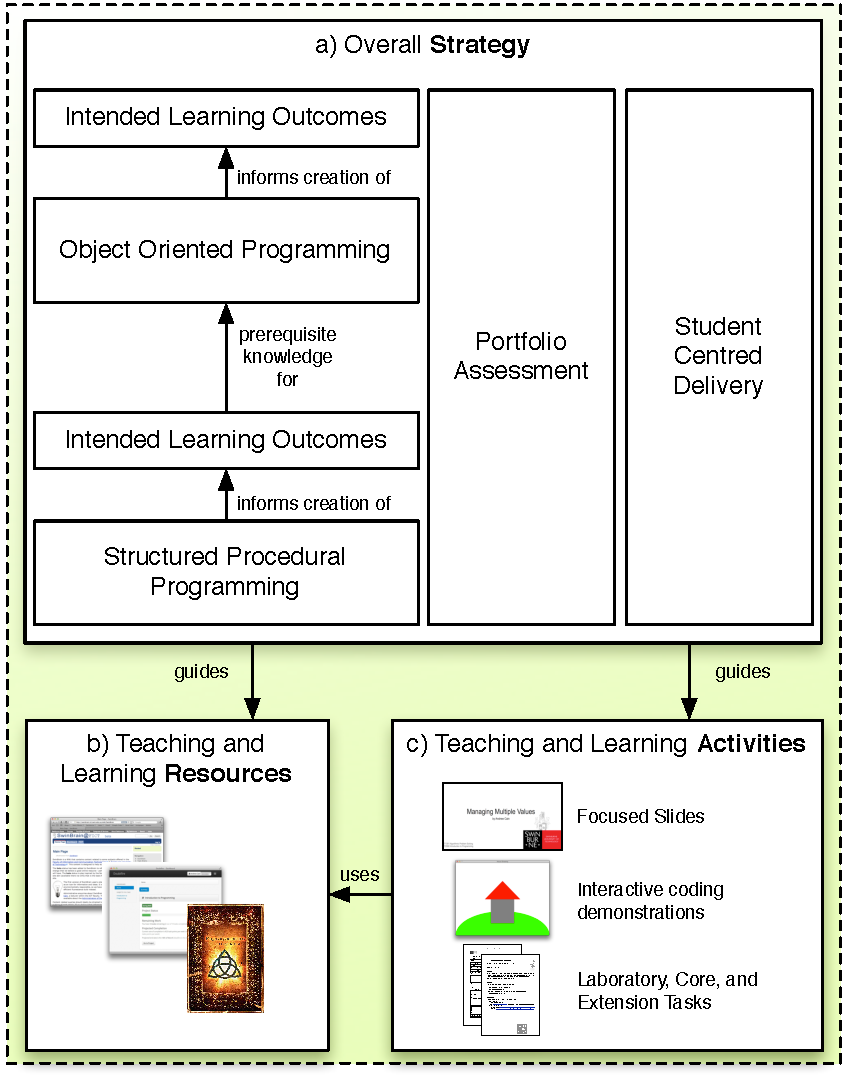
\includegraphics[width=0.77\textwidth]{OverallStrategy}
	\caption{An updated version of \fref{fig:strategy} showing the programming paradigms that will form the approach for selecting content}
	\label{fig:final_overall_strategy}
\end{figure}

\fref{fig:final_overall_strategy} shows the final overall strategy for the example units presented in this thesis. Structured procedural programming principles were used to inform the creation of the intended learning outcomes for the introductory programming unit. These outcomes then become prerequisite knowledge for the object oriented programming unit, which focused on object oriented programming principles. Both units used portfolio assessment, and focused on active student centred approaches to introducing students to unit content.


The objects-later approach taken by these example units aligns well with the principles from \cref{cha:guiding_principles}, providing a clear focus that supported a concept-based approach to introductory programming. Concepts related to object oriented programming were then the focus of the second programming unit. The alignment of these two units to the \emph{what} principles from \cref{cha:guiding_principles} is outlined in the following list.
\begin{enumerate}[noitemsep,nolistsep]
	\item The first programming unit, introductory programming discussed in \sref{sec:introductory_programming}, is aligned with the principles in the following way:
	\begin{itemize}[noitemsep,nolistsep]
		\item Content selection was guided by the structured procedural programming paradigm.
		\item Focus is on fundamental programming concepts, which include functions and procedures, variables, control flow, parameter passing, and related concepts.
		\item The chosen programming language, or languages, must have been designed for procedural programming.
	\end{itemize}
	\item The second programming unit, object oriented programming discussed in \sref{sec:object_oriented_programming}, aligns with the principles in the following way:
	\begin{itemize}[noitemsep,nolistsep]
		\item Content selection was guided by the object oriented programming paradigm.
		\item Focus is on object oriented programming concepts including abstraction, encapsulation, inheritance, and polymorphism.
		\item The chosen programming language, or languages, must have been designed for object oriented programming.
	\end{itemize}
\end{enumerate}

\clearpage
\section{Introductory Programming} % (fold)
\label{sec:introductory_programming}

\subsection{Aims for Introductory Programming} % (fold)
\label{ssub:intro:aims}

The aim of the introductory programming unit was to introduce students to programming and software development fundamentals. While the focus was on developing depth in this area, the holistic nature of the portfolio assessment approach meant that programming was placed in the context of software development in general. As a result, this unit also touched on a number of areas not traditionally associated with introductory programming such as professional ethics and communication skills.

% The following sections outline the definition of the intended learning outcomes, the construction of the assessment criteria and the development of the teaching and learning resources for the introductory programming unit.

% subsubsection aims (end)

\subsection{Defining Intended Learning Outcomes} % (fold)
\label{sec:intro:intended_learning_outcomes}

The first process in creating the introductory programming unit was to define appropriate intended learning outcomes. This was influenced by a number of factors as described in \cref{cha:approach} (see \sref{sub:defining_intended_learning_outcomes}). These factors are discussed below, and are followed by a description of the unit's intended learning outcomes that resulted.

\subsubsection{Influencing Factors} % (fold)
\label{ssub:influencing_factors}

\fref{fig:defining_ilos} shows the specific factors that influenced the definition of the introductory programming unit. Three aspects will be discussed in the following sections: the overall strategy, accreditation requirements and industry requirements. The objects-later approach meant that this unit focused on procedural programming concepts. Accreditation requirements from the Australian Computer Society (ACS) focused the content on the wider role of software development in general. Whilst the model curriculum from the Association for Computing Machinery (ACM) and Institute for Electrical and Electronic Engineers (IEEE) provided guidance from an industry perspective.

\begin{figure}[htbp]
	\centering
	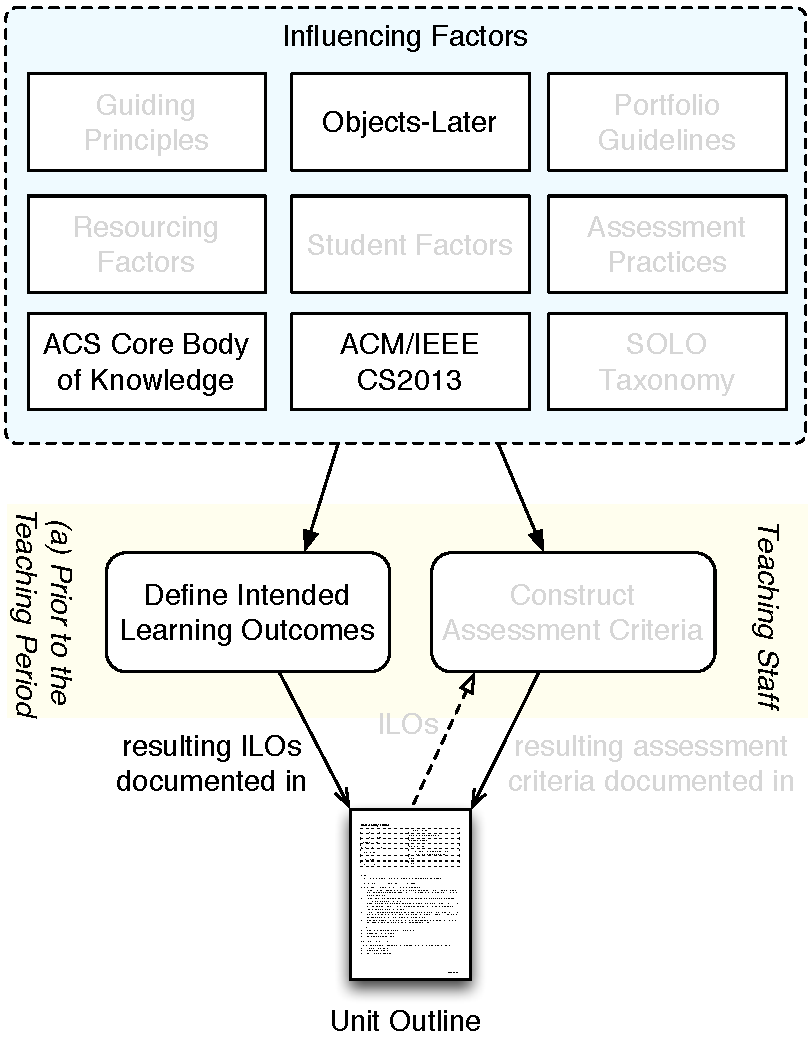
\includegraphics[width=0.65\textwidth]{ILOFactors}
	\caption{Factors that influenced the definition of the intended learning outcomes for introductory programming. Highlighting specific factors from the previous more general factors presented in \fref{fig:defining_ilos}.}
	\label{fig:defining_ilos_intro}
\end{figure}

\paragraph{Objects-Later} % (fold)
\label{par:intro:objects_later}
The objects-later approach to this unit meant that it focused on structured and procedural programming concepts. The following list outlines the core concepts that were taught in this unit.

\begin{itemize}[noitemsep,nolistsep]
	\item Procedural programming abstractions:
	\begin{itemize}[noitemsep,nolistsep]
		\item Functional abstractions: functions and procedures
		\item Data abstractions: variables, constants, arrays and types
	\end{itemize}
	\item Structured programming principles:
	\begin{itemize}[noitemsep,nolistsep]
		\item Sequence, selection and repetition
		\item Control flow: pre-test and post-test loops, if and case
		\item Iteration through an array of values
	\end{itemize}
	\item Program comprehension:
	\begin{itemize}[noitemsep,nolistsep]
		\item Memory layout: stack, heap and static memory
		\item Execution of control flow
		\item Parameter passing: pass-by-value and pass-by-reference
	\end{itemize}
\end{itemize}

% paragraph objects_later (end)

\paragraph{Accreditation Requirements} % (fold)
\label{par:accreditation_requirements}

The Australian Computer Society (ACS) documented the ICT profession and associated body of knowledge \cite{Gregor:2008}, which indicated graduates should develop both skills and knowledge as part of their undergraduate education. In the work, the skills component drew upon the Skills Framework for the Information Age (SFIA) while the knowledge area was divided into three aspects: a core body of knowledge, role specific knowledge and complementary knowledge. As a central role for a range of IT degrees, the introductory programming unit developed both student's skills and knowledge.

SFIA \cite{SFIA:2011} documented a range of IT skills across six categories. In terms of the SFIA, the Introductory Programming unit aimed to contribute to the development of \emph{programming and software development skill} from the \emph{Solution development and implementation} category. SFIA ranked each skill across seven levels of responsibility, ranging from \emph{follow} to \emph{set strategy, inspire and mobilise}. Introductory programming aimed to provide significant progress towards students attaining a Level 2, \emph{assist}, standard in this skill. To achieve this level of responsibility, students need to demonstrate the ability to design, code, test, correct, and document simple programs, as well as being able to assist with the development of larger software solutions.

The ACS divides the core body of knowledge into six areas: problem solving, professional knowledge, technology building, technology resources, service management and outcomes management. Introductory programming contributed toward the development of the problem solving, professional knowledge, technology building and technology resources as outlined in the following list:
\begin{itemize}[noitemsep,nolistsep]
	\item Problem solving:
	\begin{itemize}[noitemsep,nolistsep]
		\item Students used procedural programming abstractions, and were required to explain their various roles, properties and purpose. 
		\item Students followed methods and processes for designing and modelling procedural programming solutions.
	\end{itemize}
	\item Professional knowledge:
	\begin{itemize}[noitemsep,nolistsep]
		\item Students developed general computer competencies, including the use of compilers, shell scripting and basic Bash commands.
		\item Students read briefly about the history of computing, and the ICT discipline, providing a context for procedural programming and the structured programming principles.
		\item Professionalism, and the role of reflection and life-long learning in professional behaviour was instilled in students.
		\item Students performed self assessment of their competencies, and expertise, in applying procedural programming concepts. 
		\item The emphasis on demonstrating understanding enabled students to develop their written communication skills, including both technical and personal communications.
		\item Frequent interaction with staff aimed to help students development their interpersonal skills.
	\end{itemize}
	\item Technology building:
	\begin{itemize}[noitemsep,nolistsep]
		\item Students experienced many aspects of the software development lifecycle: undertaking simple analysis, design, implementation and testing processes.
		\item Students worked with iterative software development processes, building larger solutions across a number of iterations.
		\item The procedural programming topics listed developed practical technology building skills.
		\item An understanding of the structured programming principles helped guide program construction and evaluation.
		\item Students used simple white-box testing techniques to determine the success of their programs.
	\end{itemize}
	\item Technology resources:
	\begin{itemize}[noitemsep,nolistsep]
		\item Students developed a basic understanding of software systems, including the basics of software processes, memory layout and file systems.
	\end{itemize}
\end{itemize}

% paragraph accreditation_requirements (end)

\paragraph{Industry Requirements} % (fold)
\label{par:industry_requirements}

The Association for Computing Machinery (ACM) and IEEE Computer Society 2013 Computer Science Curriculum documents \cite{CSC2013} outlines a number of areas to be covered in a Computer Science curriculum. In terms of the ACM/IEEE model curriculum, the introductory programming unit primarily focused on \emph{Software Development Fundamentals}, but also integrated a number of other areas, as shown in the following list.

\begin{itemize}[noitemsep,nolistsep]
	\item Algorithms and Complexity:
	\begin{itemize}[noitemsep,nolistsep]
		\item \emph{Algorithmic Strategies}: Students were introduced to divide-and-conquer, and the idea of recursive backtracking.
		\item \emph{Fundamental Data Structures and Algorithms}: All students programmed simple numeric algorithms, sequential search, and basic sorting.
	\end{itemize}

	\item Computational Science:
	\begin{itemize}[noitemsep,nolistsep]
		\item \emph{Processing}: Fundamental programming concepts were covered in depth including algorithms,  implementing algorithms in code, and processes in the software development lifecycle.
	\end{itemize}

	\item Discrete Structures:
	\begin{itemize}[noitemsep,nolistsep]
		\item \emph{Basic Logic}: Students used truth tables to learn to evaluate and construct boolean expressions.
	\end{itemize}
	
	\item Graphics and Visualisation:
	\begin{itemize}[noitemsep,nolistsep]
		\item \emph{Fundamental Concepts}: Applications of computer graphics, double buffering and animation were covered to make programming more interactive.
		\item \emph{Geometric Modelling}: Optional tasks allowed students to explore procedurally generated models (fractals).
	\end{itemize}

	\item Human-Computer Interaction
	\begin{itemize}[noitemsep,nolistsep]
		\item \emph{Programming Interactive Systems}: Students developed code to manage events and user interactions.
	\end{itemize}

	\item Programming Languages:
	\begin{itemize}[noitemsep,nolistsep]
		\item \emph{Basic Type Systems}: Students explored the use of a range of basic types, along with the definition of custom enumerated and record types.
		\item \emph{Language Translation and Execution}: Students were introduced to the topics of compilers and interpreters, as well as run-time layout of memory (call-stack, heap, static data), and manual memory management.
	\end{itemize}

	\item Software Development Fundamentals
	\begin{itemize}[noitemsep,nolistsep]
		\item \emph{Algorithms and Design}: Students were introduced to the concept of algorithms, problem solving using divide-and-conquer, abstraction and program decomposition.
		\item \emph{Fundamental Programming Concepts}: Students used programming language syntax, developed programs that contained statements, expressions, used variables, simple input and output operations, conditional control flow, included functions, various parameter passing techniques, and were introduced to the concept of recursion.
		\item \emph{Fundamental Data Structures}: Programs students implemented made use of arrays, record structures, strings and basic string processing, and students implemented a simple linked list.
		\item \emph{Development Methods}: Program comprehension was central to the unit, with basic details of program correctness being introduced. Students were also required to use basic refactoring techniques to restructure code, and program tracing was covered as a debugging technique.
	\end{itemize}

	\item Software Engineering
	\begin{itemize}[noitemsep,nolistsep]
		\item \emph{Software Processes}: Students used an iterative software development process model, and were introduced to the phases of the software development lifecycle. 
		\item \emph{Software Design}: Students were introduced to the principles of the structured design paradigm, and used these principles in the design and development of the programs they created.
		\item \emph{Software Construction}: Coding standards, and defensive coding practices were introduced to students.
	\end{itemize}

	\item Social Issues and Professional Practice:
	\begin{itemize}[noitemsep,nolistsep]
		\item \emph{Professional Ethics}: Students developed skills in professional practice including self assessment, reflective practice, computer fluency, and general approaches to life-long learning.
		\item \emph{Professional Communication}: To demonstrate their understanding students were required to read, understand and communicate technical material using clear language and visual mediums.
	\end{itemize}

\end{itemize}

% paragraph industry_requirements (end)

% subsubsection influencing_factors (end)

\subsubsection{Intended Learning Outcomes} % (fold)
\label{ssub:intro_intended_learning_outcomes}

All of the factors listed above, and the factors and guidelines stated in \sref{sub:defining_intended_learning_outcomes} of \cref{cha:approach}, guided the definition of the intended learning outcomes for the introductory programming unit. The following list shows how the guidelines for defining intended learning outcomes were used in the development of the introductory programming unit.

\begin{itemize}[noitemsep,nolistsep]
	\item Verbs were selected from appropriate levels of the SOLO taxonomy. (\loref{lo-solo}) 
	\item Outcomes aimed to cover both an understanding of procedural programming concepts and applied programming skills. (\loref{lo-know-prog})
	\item Care was taken with the language used to help ensure students were able to understand each outcome. (\loref{lo-simple-terms})
	\item Only four outcomes were included. (\loref{lo-minimal})
	\item Outcomes could be met in a variety of ways, and assessed at a range of levels of understanding. (\loref{lo-general} and \loref{lo-flex})
\end{itemize}

Given the wide range of skills and knowledge mentioned, the challenge was to ensure that this could be expressed in a small number of intended learning outcomes. This task was assisted by the use of the SOLO taxonomy, and recognising that the SOLO level of each outcome indicated that earlier levels must already have been achieved.

Each outcome aimed to engage students in activities likely to help them achieve a \emph{relational} level of understanding. The verbs \emph{analyse}, \emph{apply}, \emph{construct}, \emph{implement}, \emph{interpret} and \emph{use} represent activities in which students need to use cognitive activities at the relational level of understanding. The multistructural \emph{describe} verb and the unistructural \emph{locate} verb are also used, but as a supporting activity for a higher level verb, such as with \emph{describe} and \emph{relate}.

By applying these guidelines, the resulting outcomes helped the introductory programming unit realise the following principles from \cref{cha:guiding_principles}, as previously discussed in \sref{sub:defining_intended_learning_outcomes}.

\begin{itemize}[noitemsep,nolistsep]
	\item Use of verbs at the Relational level of the SOLO taxonomy indicated the activities students needed to be able to demonstrate to pass the unit. (\Pref{itm:construct}, \Pref{itm:align}, and \Pref{itm:expectations})
	\item The small number of outcomes provided a clear focus on the concepts related to structured programming. (\Pref{itm:focus} and \Pref{itm:concepts})
	\item Flexibility in how outcomes were addressed helped to engage a wide range of student interests. (\Pref{itm:support})
\end{itemize}

The final statement of the intended learning outcomes for the introductory programming unit are listed below, with the verbs from the SOLO taxonomy indicated in bold.

\begin{guidelines}{ILO}
	\item \textbf{Apply} code reading and debugging techniques to \textbf{analyse}, \textbf{interpret}, and \textbf{describe} the purpose of program code, and \textbf{locate} within this code errors in syntax, logic, and/or good practice.
	\item \textbf{Describe} the principles of structured programming, \textbf{relate} these to the syntactical elements of the programming language used, and the way programs are developed using this language.
	\item \textbf{Construct} small programs, using the programming languages covered that include the use of arrays, functions and procedures, parameter passing with pass-by-value and pass-by-reference, custom data types, and pointers.
	\item \textbf{Use} modular and functional decomposition to break problems down functionally, \textbf{represent} the resulting structures diagrammatically, and \textbf{implement} the structure in code as functions and procedures.
\end{guidelines}

Introductory programming used a procedures-first approach, and focused on the structured programming principles of organising code using \emph{sequence}, \emph{selection} and \emph{repetition}. Students learnt to use functional and modular decomposition to break problems down, and implement solutions using functions and procedures. Data was managed using arrays and custom data types. Pointers and memory management were introduced. Various forms of parameter passing were covered, including pass-by-value and pass-by-reference. Weaved through this was an iterative development process, a focus on writing clear and legible code, and other good programming practices. In addition to writing code, students learnt to read code for the debugging purposes, and to demonstrate their ability to interpret other peoples code.

Other factors, not directly stated as intended learning outcomes, were incorporated in the unit as a means of addressing wider graduate attributes, or as beneficial outcomes not directly assessed in determining the final student grades. This included professional communication, software engineering methods and graphics and visualisation.

\paragraph{Professional Communication} % (fold)
\label{par:professional_communication}

Traditionally, many programming units have focused on assessing code outcomes, assuming that if students could produce code, they understood it. Others, such as \citet{Lister:2004}, extended this to include small code reading and tracing tasks in order to expand on the assessment of student's understanding of code. 

With the example introductory programming unit this is taken further, with the students needing to write about the associated principles and to describe code. This expanded assessment had the dual benefit of engaging higher levels of cognitive activity, while also helping students to develop their professional communication skills.

Each of the intended learning outcomes requires students to communicate their understanding. For example, in meeting the first outcome students needed to demonstrate the ability to interpret supplied code, and to communicate its purpose and any issues in logic or the application of recommended good practice. While not a direct focus of the assessment, communication skills play an enabling role in achieving this, and students were provided with support and encouragement in developing their communication skills alongside their technical skills.

% paragraph professional_communication (end)
 
\paragraph{Software Engineering Methods} % (fold)
\label{par:software_engineering_methods}

While typically the focus of later software engineering units, the software development lifecycle and iterative development methods were embedded within the unit. Students engaged in the development of software throughout the unit: analysing, designing, developing and testing software became a means for them to achieve these outcomes. Students experienced the software development lifecycle first hand, without needing it to be stated in the unit's intended learning outcomes.

Larger programs in the unit were broken down into a number of iterations, and students build these solutions by performing these iterations. Once again, this enabled them to experience software development methods without these methods being explicitly included in the assessed outcomes.

Together, both of these aspects were related to the more general concept of \emph{problem decomposition}. The idea of approaching a solution through discrete iterations provided an example of decomposing a problem into smaller steps. Similarly, the idea of breaking each of these steps into more manageable processes was used to explain both the idea of decomposition and the software development lifecycle. 

% paragraph software_engineering_methods (end)

\paragraph{Graphics and Visualisation} % (fold)
\label{par:graphics_and_visualisation}

Identifying appropriate applications for student to develop is a common problem with teaching introductory programming. In teaching introductory programming it was decided to focus on having students program small computer games. The research literature related to the use of games indicates that this is popular with students \cite{Bayliss:2006}, and helps motivate them to spend time on the task \cite{Feldgen:2004,Rajaravivarma:2005,Cliburn:2006}, as well as supporting development of student understanding of programming concepts \cite{Roberts:1995,Leutenegger:2007}.

% \begin{itemize}[noitemsep,nolistsep]
% 	\item \citet{Roberts:1995} used a graphical library in teaching introductory programming and reported that it enhanced student interest and reinforced essential programming concepts.

% 	\item \citet{Feldgen:2004} reported their highest class attendance for the unit after shifting to using games, with improvements in pass rates and student retention.

% 	\item The greenfoot environment, introduced in \citet{Kulling:2005}, was created to help introduce high school students to object oriented programming.

% 	\item \cite{Rajaravivarma:2005} used text-based and numeric games as a domain for introductory programming and indicated the approach created a ``passion to want to do more.''

% 	\item \citet{Bayliss:2006} discussed the use of games in a summer distance unit introducing students to programming and concepts in computer science. The work reported that a large percentage of students enjoyed learning introductory programming concepts in the context of games.

% 	\item Results from \citet{Cliburn:2006} suggested that for a large majority of students games had provided psychological motivation and had increased unit enjoyment.

% 	\item \citet{Leutenegger:2007} reported that games had improved student understanding of all basic topics examined.

% 	\item \citet{Sung:2009} provided some guidelines on incorporating games into introductory programming. This indicated a need to ensure tools are freely available, that core concepts need to remain the focus, and that games should aim to be gender and expertise neutral.

% 	\item \citet{Sung:2011} introduced a number of game-themed programming assignments to help other teaching staff make the transition to game based introductory programming.

% \end{itemize}

The use of games as a context for software development requires students to gain some familiarity with fundamental concepts related to graphics and animation. The interactive nature of games also introduces students to the concept of programming in response to user input events and real-time signals.

% paragraph graphics_and_visualisation (end)
\clearpage
\subsection{Constructing Assessment Criteria} % (fold)
\label{sub:intro_constructing_assessment_criteria}

The construction of the assessment criteria happened alongside the definition of the intended learning outcomes. The goal, as stated in \sref{sub:constructing_assessment_criteria} of \cref{cha:approach}, was to create clearly distinct grades where each required students to demonstrate a deeper understanding of programming concepts and software development practices. These goals were met by applying the guidelines from \cref{cha:approach} as outlined in the following list.

\begin{itemize}[noitemsep,nolistsep]
	\item Simple language was used to describe the various levels to which the outcomes could be met. (\acref{ac-simple-terms})
	\item Pass and higher grades required students to demonstrate how they had met each of the unit's intended learning outcomes. (\acref{ac-all-ilos})
	\item Critieria for grades higher than Pass required student to demonstrate deeper understanding of the concepts related to the intended learning outcomes. (\acref{ac-grades})
	\item Each grade required distinct evidence. (\acref{ac-distinct})
	\item A clear mapping was provided from the assessment criteria to grade outcomes, and was provided in the unit outline. (\acref{ac-map})
\end{itemize}


\fref{fig:assessment_criteria} shows the assessment criteria developed for the introductory programming unit. To receive a \emph{Pass} or \emph{Credit} grade, students completed set exercises, which were signed off through student interaction with staff. \emph{Distinction} required the implementation of a program of the student's own creation, while \emph{High Distinction} required a small research project.

\begin{figure}[p]
	\centering
	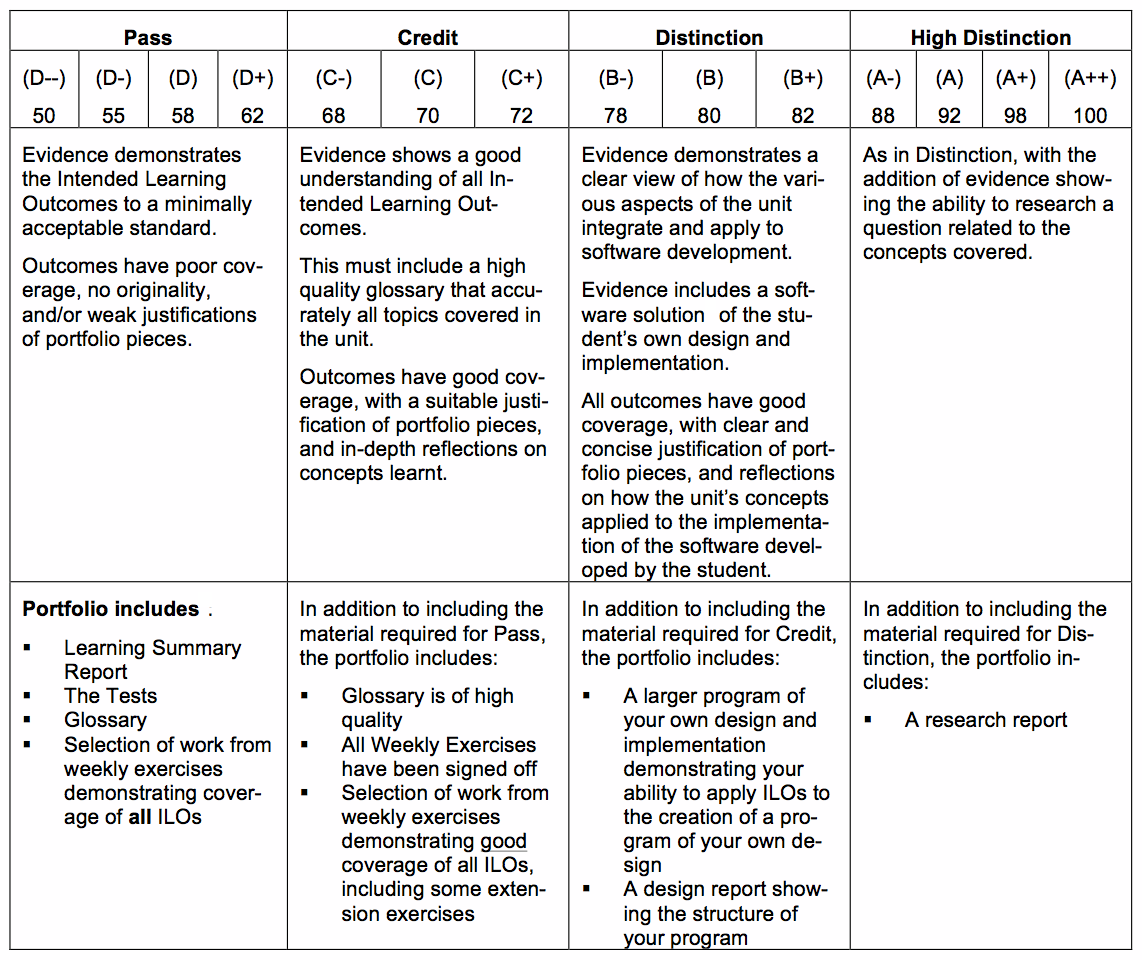
\includegraphics[width=\textwidth]{AssessmentCriteria}
	\caption{Assessment criteria from the Unit Outline of the introductory programming unit}
	\label{fig:assessment_criteria}
\end{figure}

\begin{figure}[p]
	\centering
	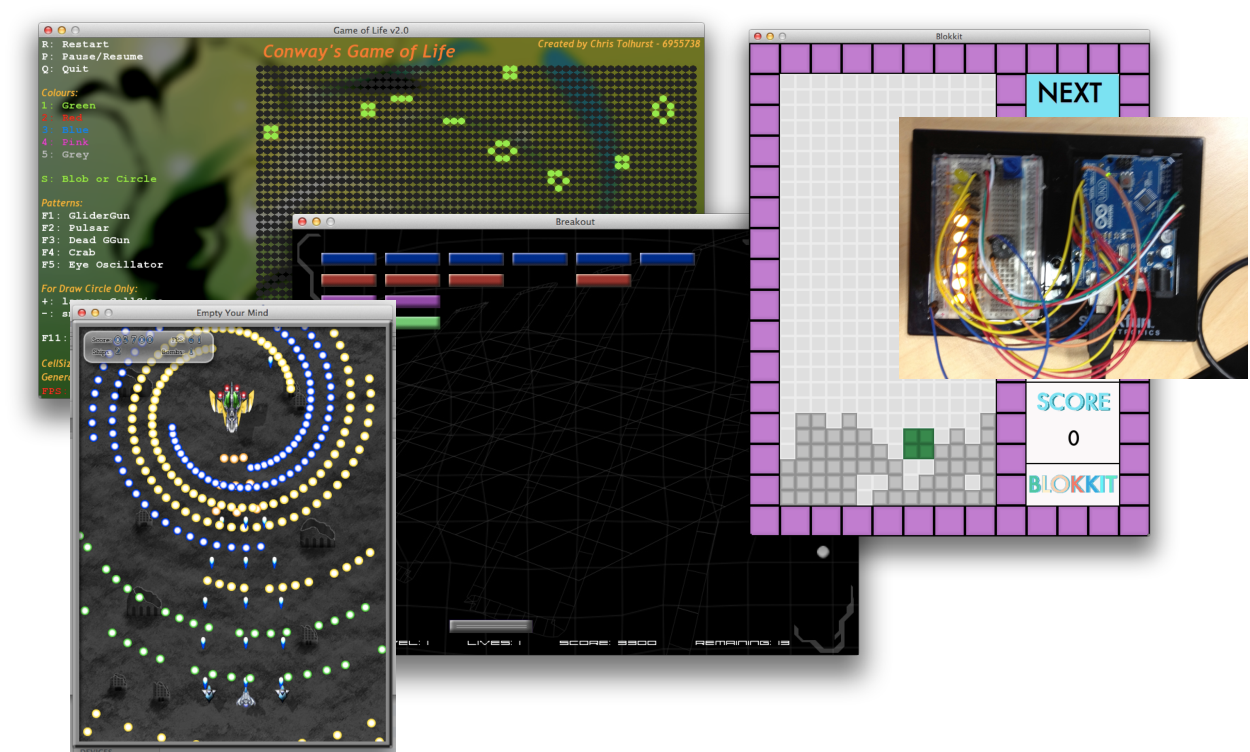
\includegraphics[width=0.9\textwidth]{StudentGames}
	\caption{Example images of student work, including screenshots of games and a photograph of hardware components.  }
	\label{fig:student_games}
\end{figure}

To receive at least a \emph{Pass} grade, students needed to satisfactorily complete three hurdle tests as well as a number of pieces of work that demonstrated they had met all of the intended learning outcomes. These pieces of work needed to come from the weekly tasks, but did not need to have been signed off by teaching staff. 

The \emph{Credit} grade required students to meet all Pass requirements, and to have succeeded in getting all tasks signed off. This ensured teaching staff were happy they had completed the work themselves and provided students with incentives to engage in the formative feedback process. Students' explanations of programming concepts and abstractions were the main items used to distinguish between Pass and Credit in terms of depth of understanding. In this regard, the student's work needed to demonstrate good coverage of all outcomes for the student to be eligible for a Credit grade.

\emph{Distinction} built on top of Credit requirements and required students to create a program of their own design. This could be any program the student was interested in creating, as long as it demonstrated good coverage of all of the unit's intended learning outcomes. In effect, this meant that students needed to create a program that contained a number of functions and procedures, used arrays and record types, and was of sufficient size and complexity. Most students who received this grade had implemented a game of some kind, many emulating classic arcade games such as asteroids, pong, frogger or space invaders. However others implements small databases, and in a couple of cases implemented programs for custom hardware. \fref{fig:student_games} shows a number of images of student work, including a number of games and one piece of custom hardware.

\emph{High Distinction} required students to engage in the creation of a short research report, in addition to having met the Distinction grade requirements. Each student aiming to achieve this grade worked together with staff to define a topic they could examine, and then the student carried out data collection, analysis and reporting tasks. As an introductory programming unit, this research was limited to examining simple tasks such as algorithm efficiency, different techniques to perform a task, or comparing performance aspects of different code. Students were encouraged to think deeply about their results, and to document their outcomes clearly.

As indicated in \sref{sub:constructing_assessment_criteria}, the use of these assessment criteria in the introductory programming unit helped it to embody the following principles from \cref{cha:guiding_principles}:

\begin{itemize}[noitemsep,nolistsep]
	\item Criteria for Credit, Distinction, and High Distinction grades required progressively higher levels of understanding which promoted deep learning, and communicated high staff expectations. (\Pref{itm:construct} and \Pref{itm:expectations})
	\item Students needed to demonstrate understanding across all outcomes. (\Pref{itm:align})
	\item The criteria determined each student's final grade, delaying all summative assessment until the end of the unit and encouraging students integrate feedback they received. (\Pref{itm:formative} and \Pref{itm:agile})
	\item Different levels in the assessment criteria focused on addressing the most important aspects for students to focus on. (\Pref{itm:focus})
	\item As with the learning outcomes, the use of simple terms helped support a wide range of student language capabilities. (\Pref{itm:support})
	\item Clearly distinct requirements helped students take responsibility for their learning, allowing them to aim to meet certain grade criteria. (\Pref{itm:theory_y})
	\item Students reflected on their learning in preparing their portfolios. (\Pref{itm:reflect})
	\item Students needed to demonstrate appropriate use of procedural programming concepts, and programming languages. (\Pref{itm:paradigm}, \Pref{itm:concepts} and \Pref{itm:authentic})
\end{itemize}

% subsection constructing_assessment_criteria (end)

\subsection{Developing Teaching and Learning Activities} % (fold)
\label{sub:intro_developing_teaching_and_learning_activities}

\sref{ssub:develop_teaching_and_learning_activities_and_resources} of \cref{cha:approach} provided three guidelines to inform the development of teaching and learning activities. These indicated that teaching and learning activities should actively engage students (\tlaref{itm:tla_active}), align with unit outcomes (\tlaref{itm:tla_align}), and focus on providing guidance rather than aiming to transfer knowledge (\tlaref{itm:tla_focus}). All of these guidelines were adopted in the development of the teaching and learning activities for the introductory programming unit.

Allocated classes for this thirteen week introductory programming unit included a two hour lecture, and a two hour laboratory class each week. All classes were designed with the goal of actively engaging students, as discussed in \sref{sub:delivery_approach}. A typical lecture included a short presentation using ``Beyond Bullet Points'' style lecture slides \cite{Atkinson:2007}, an interactive programming demonstration and group activities. In the laboratory sessions, students were involved in code reading activities, guided programming tasks and practical hands-on exercises.

The teaching period consisted of twelve teaching weeks, and a single week semester break. Topics for the twelve lectures are shown in the following list. In weeks one to six students explored these concepts using a modern version of the Pascal programming language \cite{Wirth:1971,FPC:2011}. To help reinforce the applicability of the programming concepts across programming languages, students were introduced to the C programming language \cite{Ritchie:1978} in week 7, and this language was used for the remainder of the semester. 

\begin{enumerate}[noitemsep,nolistsep]
  \item Programs, Procedure, Compiling and Syntax
  \item User Input and Working with Data
  \item Control Flow: Branches and Loops
  \item Procedural and Structured Programming
  \item Arrays
  \item Custom Data Types and Pointers
  \item Learning a New Language
  \item Programming in C
  \item File Input and Output
  \item Dynamic Memory Management
  \item Recursion and Backtracking
  \item Review and Future Studies
\end{enumerate}

Each week's laboratory class consisted of a number of activities. At the start of the class the teaching staff returned the feedback from the previous week's core exercises, but delayed discussing feedback with students until after working through the exercises. Students where then guided through the week's laboratory exercises, and the core exercises were discussed. Students spent the remaining laboratory time on the week's core exercises. During this time the teaching staff visited each student individually to discuss their progress, and to mark their work as signed off. At the end of laboratory classes students were reminded of the tasks they needed to complete by the following week, and encouraged to attempt extension tasks.

To provide students with an opportunity to demonstrate their understanding, each week's core exercises also had students developing a detailed glossary. For the introductory programming unit, the glossary had students record details on the following topics:
\begin{itemize}[noitemsep, nolistsep]
	\item Core concepts:
	\begin{itemize}[noitemsep, nolistsep]
		\item Control flow
		\item Structured programming principles
		\item Functional and modular decomposition
		\item Good programming practices
	\end{itemize}
	\item Programming terminology:
	\begin{itemize}[noitemsep, nolistsep]
		\item Statements
		\item Expressions
		\item Identifiers
		\item Parameters, local variables and global variables
	\end{itemize}
	\item Programming abstractions:
	\begin{itemize}[noitemsep, nolistsep]
		\item Programs
		\item Functions and Procedures
		\item Constants and Variables
		\item Arrays
		\item Records and Enumerations
		\item Pointers
	\end{itemize}
	\item Statements:
	\begin{itemize}[noitemsep, nolistsep]
		\item Function and procedure calls
		\item Assignment statements
		\item If and case statements
		\item While and repeat/do..while loops
		\item For loops
	\end{itemize}
\end{itemize}

\tref{tbl:intro_prog_matrix} shows the planned alignment between the introductory programming unit's topics and its intended learning outcomes. This planned alignment was not shared with students to ensure that their portfolios reported how \emph{they} believed the tasks aligned with the outcomes. In this way, the process of alignment was carried out by both staff \emph{and} students -- teaching staff planned activities they believed aligned with outcomes, while students reflected on their learning experience and reported how their work demonstrated they had met the outcomes. 

\begin{table}[b]
	\centering
	\caption{Alignment matrix showing staff-planned alignment of weekly topics to the introductory programming unit's intended learning outcomes. Student descriptions of the topic alignment differed based on their individual learning.}
	\label{tbl:intro_prog_matrix}
	\footnotesize
	\begin{tabular}{l|cccc}
		\textbf{Topic} 								& \textbf{ILO-1} & \textbf{ILO-2} & \textbf{ILO-3} & \textbf{ILO4} \\ \hline
		Programs, Procedure, Compiling and Syntax 	& \checkmark & \checkmark & \checkmark & \checkmark \\ 
		User Input and Working with Data 			& \checkmark & \checkmark & \checkmark & \checkmark \\
		Control Flow: Branches and Loops 			& \checkmark & \checkmark & \checkmark & ~ \\
		Procedural and Structured Programming 		& \checkmark & \checkmark & \checkmark & \checkmark \\	
		Arrays 										& \checkmark & \checkmark & \checkmark & ~ \\
		Custom Data Types and Pointers 				& \checkmark & ~ & \checkmark & ~ \\
		Learning a New Language 					& \checkmark & \checkmark & \checkmark & \checkmark \\
		Programming in C 							& \checkmark & \checkmark & \checkmark & \checkmark \\
		File Input and Output 						& ~ & ~ & \checkmark & ~ \\
		Dynamic Memory Management 					& \checkmark & ~ & \checkmark & ~ \\
		Recursion and Backtracking 					& \checkmark & ~ & \checkmark & ~ \\
		Review and Future Studies 					& \checkmark & \checkmark & \checkmark & \checkmark \\
	\end{tabular}
\end{table}

By following the guidelines from \sref{ssub:develop_teaching_and_learning_activities_and_resources}, the teaching and learning activities in the introductory programming unit addressed a number of the principles stated in \cref{cha:guiding_principles}. 

\begin{itemize}[noitemsep,nolistsep]
	\item Activities aimed to actively engaged students in tasks likely to engage the required cognitive levels. (\Pref{itm:construct})
	\item Staff planned activities they believed would enable the students to demonstrate they had met the unit's intended learning outcomes. (\Pref{itm:align}) 
	\item Activities supported the use of weekly formative feedback, providing tasks over which staff and students could have meaningful dialogue. (\Pref{itm:formative} and \Pref{itm:theory_y})
	\item Activities focused on concepts, providing students with a range of opportunities to develop pieces that would demonstrate they had gained the required knowledge. (\Pref{itm:focus}, \Pref{itm:support} and \Pref{itm:concepts})
	\item Core and extension tasks helped to communicate staff expectations. (\Pref{itm:expectations})
	\item Leaving language details to be covered in teaching and learning resources helped to ensure activities could change in response to student needs. (\Pref{itm:agile})
	\item Activities ensured students implemented a range of procedural programs, making use of programming languages in ways in which they were intended. (\Pref{itm:paradigm} and \Pref{itm:authentic})
\end{itemize}

\clearpage
\subsubsection{Procedures First Topic Sequence} % (fold)
\label{ssub:procedures_first_topic_sequence}

The order of topics was guided by \pref{itm:concepts} from \cref{cha:guiding_principles}. The main objective being to enable each week's topic to build upon earlier topics, while providing a consistent set of abstractions for students to work with.

This was achieved using a procedures-first approach in which students program their own procedures from Week 1. The following list indicates the concepts, programming abstractions and statements introduced each week.

\begin{enumerate}[noitemsep,nolistsep]
  \item Programs, Procedure, Compiling and Syntax
  \begin{itemize}[noitemsep,nolistsep]
  	\item \textbf{Sequence}: The focus of this week was on programs and procedures as a \emph{sequence} of instructions that get the computer to perform a task.
  	\item \textbf{Syntax Rules}: Students learnt to use visual ``railroad'' diagrams \cite{Braz:1990} to understand programming language syntax.
  	\item \textbf{Program}: Students created small programs that contained a sequence of procedure calls, with all values being hard coded.
  	\item \textbf{Procedure}: Students developed a small number of procedures, each with a defined task that contributed to the overall program.
  \end{itemize}
  \item User Input and Working with Data
  \begin{itemize}[noitemsep,nolistsep]
  	\item \textbf{Data}: The central idea of this week was \emph{data}, the idea that values can be stored and calculated.
  	\item \textbf{Variables}: Students created local variables, global variables and parameters.
  	\item \textbf{Constants}: Students declared constants.
  	\item \textbf{Functions}: Students used functions in the laboratory and core exercises, and developed their own in the extension tasks.
  	\item \textbf{Assignment Statements}: Students used assignment statements to store values in variables. 
  \end{itemize}
  \item Control Flow: Branches and Loops
  \begin{itemize}[noitemsep,nolistsep]
  	\item \textbf{Control Flow}: The ideas of sequence, selection and repetition were central to this week.
  	\item \textbf{Selection}: Students used \textbf{if statements} and  \textbf{case statements} to implement branching in their control flow.
  	\item \textbf{Repetition}: Students repeated code using \textbf{while loops} and \textbf{repeat loops}.
  \end{itemize}
  \item Procedural and Structured Programming
  \begin{itemize}[noitemsep,nolistsep]
  	\item \textbf{Functional and Modular Decomposition}: The idea of solving problems using divide-and-conquer was the main theme of this week.
  	\item \textbf{Software Development Lifecycle}: The basic steps of the software development lifecycle were discussed.
  	\item \textbf{Iterative Development}: The idea of iteratively working toward a solution was discussed.
  	\item \textbf{Structured Programming}: The structured nature of a functions/procedures code was discussed, illustrating how these steps can be broken down into blocks performing sequence, selection or repetition.
  	\item No new programming abstractions or statements were introduced in this week.
  \end{itemize}
  \item Arrays
  \begin{itemize}[noitemsep,nolistsep]
  	\item \textbf{Arrays}: Students started to use arrays to store multiple values in their programs.
  	\item \textbf{For loops}: The for loop was introduced as a convenient means of looping through the contents of an array, allowing the code to easily apply a set of operations on each element in the array.
  \end{itemize}
  \item Custom Data Types and Pointers
  \begin{itemize}[noitemsep,nolistsep]
  	\item \textbf{Types}: Custom types and the role of types in a programming languages were discussed.
  	\item \textbf{Records}: Students developed their own custom record types to model entities associated with their programs.
  	\item \textbf{Enumerations}: Students use of enumerations as a means of creating a type to represent a list of options.
  	\item \textbf{Pointers}: Pointers were used to create relationships between values, and to illuminate how pass-by-reference worked internally.
  \end{itemize}
  \item Learning a New Language
  \begin{itemize}[noitemsep,nolistsep]
  	\item \textbf{Language Syntax}: Ways to approach a new programming language were discussed, and students used a new language to recreate previously developed programs.
  \end{itemize}
  \item Programming in C
  \begin{itemize}[noitemsep,nolistsep]
  	\item No new programming concepts or abstractions were presented in this week. Instead the week was used to consolidate knowledge of the new language, and to develop a wider range of programs using the previously presented concepts.
  \end{itemize}
  \item File Input and Output
  \begin{itemize}[noitemsep,nolistsep]
  	\item \textbf{File Input and Output}: The idea of persisting data was presented, and students learnt to save data to a file and read it back. 
  \end{itemize}

  \item Dynamic Memory Management
  \begin{itemize}[noitemsep,nolistsep]
  	\item \textbf{Stack and Heap}: Specifics related to memory layout were discussed, including the limitations of the stack.
  	\item \textbf{Dynamic Memory Allocation}: Students used memory allocation functions to allocate memory from the heap, and used pointers to work with the newly allocated space.
  \end{itemize}

  \item Recursion and Backtracking
  \begin{itemize}[noitemsep,nolistsep]
  	\item \textbf{Recursion}: Students developed simple recursive solutions for problems like the Fibonacci sequence and the Towers of Hanoi.
  	\item \textbf{Backtracking}: The idea that a recursive solution can backtrack to search alternative paths was discussed, and extension tasks introduced backtracking to solve Sudoku and the Eight Queens puzzle.
  \end{itemize}

  \item Review and Future Studies
  \begin{itemize}[noitemsep,nolistsep]
  	\item This week did not introduce any new programming concepts or abstractions, instead it was used to review everything that had been covered and to discuss future programming units.
  \end{itemize}
\end{enumerate}

\citet{Pattis:1990,Pattis:1993} indicated that the main challenge with the procedures first approach was that students did not have anything meaningful to program in their procedures prior to introducing control flow. \citet{Pattis:1993} reported that the majority of procedures-first texts had moved control flow prior to procedure declarations in response to this issue. We took an alternative approach, and introduced students to a game development framework in Week 1. This framework provided a range of useful procedures that students could call, and thereby addressed the issues that Pattis had raised. Details of this game development framework are presented in \cref{cha:supporting}.

The following list outlines the focus of each week's tasks.
\begin{enumerate}[noitemsep,nolistsep]
  \item Programs, Procedure, Compiling and Syntax
  \begin{itemize}[noitemsep,nolistsep]
  	\item \textbf{House Drawing}: Students created a procedure to draw a house at a fixed location on the screen, using a sequence of procedure calls. 
  	\item \textbf{Knock Knock}: Students created a number of procedures to show images and play sound effects necessary to display a knock knock joke.
  	\item \textbf{Custom Splash}: Extensions encouraged students to develop a procedure to show their own splash screen.
  \end{itemize}
  \item User Input and Working with Data
  \begin{itemize}[noitemsep,nolistsep]
  	\item \textbf{House Drawing}: Redeveloped to make use of parameters and local variables, allowing the house position to be changed.
  	\item \textbf{Bike Drawing}: Students developed a procedure to draw a fixed size bike, using parameters for the bike's location and colour.
  \end{itemize}
  \item Control Flow: Branches and Loops
  \begin{itemize}[noitemsep,nolistsep]
  	\item \textbf{Lots of Bikes}: Students created a custom screen saver like program that drew thousands of bikes to the screen.
  	\item \textbf{Circle drawing}: Students developed a program in which they could move a circle around the screen, switching it between outlined and filled modes, and mouse clicking it to make the circle jump to a random position.
  \end{itemize}
  \item Procedural and Structured Programming
  \begin{itemize}[noitemsep,nolistsep]
  	\item \textbf{User input functions}: Students created functions to read strings, integers, doubles, and ranges of values (between a minimum and maximum) from the user. These build on top of each other to demonstrate the power of functional decomposition.
  	\item \textbf{Arcade game}: Students were encouraged to develop a simple clicking arcade game using the concepts already covered.
  \end{itemize}
  \item Arrays
  \begin{itemize}[noitemsep,nolistsep]
  	\item \textbf{Statistics}: Students developed a program that read in a number of values from the user and then calculated various statistic values. This included median, which required the values in the array to be sorted.
  \end{itemize}
  \item Custom Data Types and Pointers
  \begin{itemize}[noitemsep,nolistsep]
  	\item \textbf{Address Book}: A simple address book, with links to friends was developed to demonstrate records and pointers.
  	\item \textbf{Pop Game}: Provided a larger, multiple iteration, project in which students developed a simple arcade style game. The game involved popping different kinds of shapes, with rounds of ten shapes each of random sizes and colours.
  \end{itemize}
  \item Learning a New Language
  \begin{itemize}[noitemsep,nolistsep]
  	\item \textbf{User Input Functions}: Students redeveloped the user input functions using the new programming language. 
  \end{itemize}
  \item Programming in C
  \begin{itemize}[noitemsep,nolistsep]
  	\item \textbf{Statistics} was reimplemented in the new programming language.
  \end{itemize}
  \item File Input and Output
  \begin{itemize}[noitemsep,nolistsep]
  	\item \textbf{Address Book} was reimplemented in C, and added the ability to save it to file, and load it from file. 
  \end{itemize}

  \item Dynamic Memory Management
  \begin{itemize}[noitemsep,nolistsep]
  	\item \textbf{Address Book}: Dynamic memory management was used to allow for a variable number of contacts in the address book.
  	\item \textbf{Maze Game}: Extension tasks had the students develop a network of rooms connected using pointers.
  \end{itemize}

  \item Recursion and Backtracking
  \begin{itemize}[noitemsep,nolistsep]
  	\item \textbf{Recursive Programs}: Extension tasks had students develop recursive functions.
  	\item \textbf{Linked List}: Extension tasks demonstrated how to use pointers and records/structures to create a linked list.
  \end{itemize}

  \item Review and Future Studies
  \begin{itemize}[noitemsep,nolistsep]
  	\item There was no lab exercises this week, and the lab was used to help students complete any outstanding tasks.
  \end{itemize}
\end{enumerate}

% subsubsection procedures_first_topic_sequence (end)

\subsubsection{Programming Language Choice} % (fold)
\label{ssub:programming_language_choice}

Introductory programming aimed to teaching students to \emph{program}, not the details of a programming language. We did not aim to develop students' expertise in one programming language, but to equip them with the knowledge and skills to become proficient in \textbf{any} imperative programming language.

Whenever discussing introductory programming it is always interesting to note how quickly people jump to the question of language. In the delivery of this unit the programming language was always a secondary concern -- an enabling feature -- not an aspect of great importance. The language choice was based on its ability to support the following requirements:
\begin{itemize}[noitemsep,nolistsep]
	\item \textbf{Explicit} \emph{over} implicit
	\begin{itemize}[noitemsep,nolistsep]
		\item Require explicit variable declaration, with clear indication of the variable's type.
		\item Strongly typed, avoiding implicit type conversions.
	\end{itemize}

	\item \textbf{Procedural programming abstractions} \emph{over} support for other paradigms.
	\begin{itemize}[noitemsep,nolistsep]
		\item Functions and procedures.
		\item Pass-by-value and pass-by-reference.
		\item Arrays, constants and variables.
		\item Declaration of custom types including enumerations and record structures.
		\item Pointers and dynamic memory management.
	\end{itemize}
\end{itemize}

\begin{table}[hb]
	\renewcommand{\arraystretch}{1.6}
	\centering
	\caption{Comparison of programming languages for the introductory programming unit.}
 	\label{tbl:language_comparison}
 	\small
    \begin{tabular}{l|c|c|c|c|c|c}
    ~                                   & C   & C++ & C\#     & Java & Pascal & Python \\ \hline
    Explicit Variables                  & \checkmark & \checkmark & \checkmark     & \checkmark  & \checkmark    & ~      \\
    Strongly Typed                      & ~   & ~   & \checkmark     & \checkmark  & \checkmark    & \checkmark    \\
    Functions and procedures            & \checkmark & \checkmark & Partial & ~    & \checkmark    & \checkmark    \\
    Parameter passing options & ~   & \checkmark & \checkmark     & ~    & \checkmark    & ~     \\
    Data abstractions     & \checkmark & \checkmark & \checkmark     & \checkmark  & \checkmark    & \checkmark    \\
    Records and enumerations  & \checkmark & \checkmark & \checkmark     & ~    & \checkmark    & ~      \\
    Pointers                            & \checkmark & \checkmark & Partial & ~    & \checkmark    & ~      \\
    Explicit memory management & \checkmark & \checkmark & ~ & ~    & \checkmark    & ~      \\
    Used by staff     & \checkmark & \checkmark & \checkmark     & \checkmark  & \checkmark    & \checkmark    \\
    \end{tabular}
\end{table}

\tref{tbl:language_comparison} lists the languages considered for the introductory programming unit. Pascal met all of the requirements, with C++ and C\# satisfying most. C\# was designed for object oriented programming, and therefore using it for procedural programming was against \pref{itm:authentic}, which indicated we would only use languages as they were designed to be used. 

The choice between C++ and Pascal was more challenging. C++ had the advantage of being widely used, and the popularity of the C-style syntax would mean that learning its syntax would more directly help students when with these other languages. However, the C++ language itself is cryptic and would be more challenging for students to master on their own. Pascal, on the other hand, was seen as having a more ``beginner friendly'' syntax. Pascal had also been used by \citet{Becker:2002}, who stated that it had enabled them to focus less on the syntax, as compared to C++.

Rather than choosing \emph{one} language it was decided to take advantage of both languages. Students would be able to focus more on the concepts using Pascal's more friendly syntax over the first few weeks of the semester. Once all the concepts were covered the language could be switched and students could explore the procedural aspects of C++, getting a start with a C-style syntax.

The focus on teaching students to ``understanding syntax'' from Week 1 supported, and was supported by, the change of language. Students had been exposed to programming language syntax using the visual ``railroad'' diagram syntax notation \cite{Braz:1990}, and had used this to learning Pascal over the first weeks of the unit. After the switch to C++, students could reinforce these same skills by applying them to learn a second programming language. Students again consulted railroad diagrams as they learnt the C syntax themselves. This approach aimed to encourage students to focus on the concepts, which would then enable them to more quickly learning the new language.

% subsubsection programming_language_choice (end)

% subsection developing_teaching_and_learning_activities (end)


\subsection{Delivering the Unit} % (fold)
\label{sub:delivering_the_unit}

Delivery of the unit followed the iterative delivery process outlined in \sref{ssub:deliver_unit} of \cref{cha:approach}, and used the activities outlined in the previous section. The process involved the delivery of lectures to guide student activity, used resources to provide students with details, provided weekly formative feedback on assessment tasks, which students then incorporated to improve their understandings. The following list outlines how the guidelines from \sref{ssub:deliver_unit} were adopted, with additional details provided in the following paragraphs.

\begin{itemize}
	\item Lecture and laboratory classes aimed to actively engage students, as described in \sref{sub:intro_developing_teaching_and_learning_activities}. (\iduref{itm:idu_active} and \iduref{itm:idu_align})
	\item Students submitted work weekly for formative feedback, with the portfolio being the only work that contributed to the students' grades. (\iduref{itm:idu_formative}) 
	\item An online discussion board and Programming Help Desk were used to actively support students throughout the teaching period. (\iduref{itm:idu_support})
\end{itemize}

Each week the lecture presented the relevant concepts, with demonstrations introducing students to the syntax. Laboratory sessions helped students prepare for the core tasks, which they completed after each class. Completed core and extension tasks were submitted for formative feedback at the start of subsequent lectures and the process repeated across each week of the teaching period.

With lectures providing guidance, and laboratories getting students started with a topic, students often had questions outside of scheduled class times. These were supported via a Programming Help Desk and an online discussion board. The Programming Help Desk was available to students during the week, and was staffed by later year students and teaching staff from the unit. Students were encouraged to drop in to the help desk to seek clarification on any issues they had with the concepts or programming language syntax. The unit also made heavy use of the university's online learning management system to provide additional support for students outside of scheduled class times. The use of the discussion board was actively encouraged, and questions were promptly answered by teaching staff, and in some cases by fellow students.

Delivering the introductory programming unit in this way ensured it met all of the principles stated in \cref{cha:guiding_principles}, as outlined in the following list. 
\begin{itemize}[noitemsep,nolistsep]
	\item Students were actively engaged in constructing their own knowledge as they worked through the teaching and learning activities. (\Pref{itm:construct})
	\item Activities provided opportunities for students to develop pieces of work that aligned to the unit's intended learning outcomes. (\Pref{itm:align})
	\item Weekly tasks were used to provide frequent formative feedback, with students actively being encouraged to incorporate the feedback to improve their work and understanding. (\Pref{itm:formative})
	\item Activities had a clear focus: lectures providing guidance, laboratory classes a first exposure, and support structures providing assistance outside of scheduled class times. (\Pref{itm:focus})
	\item Weekly tasks, along with extensions, helped communicate high staff expectations. (\Pref{itm:expectations})
	\item The discussion board and Programming Help Desk provided active support for students in addition to scheduled class times. (\Pref{itm:support})
	\item Student had to take responsibility for their learning, no marks were attached to any of the weekly work so as to ensure it retained its formative focus. (\Pref{itm:theory_y})
	\item Execution of teaching and learning activities provided insights that could be feed back into the reflective agile process, ensuring changes helped address student needs.  (\Pref{itm:agile} and \Pref{itm:reflect})
	\item The concepts central to the unit focused on structured procedural programming. (\Pref{itm:paradigm} and \Pref{itm:concepts})
	\item Students used the Pascal and C programming languages in ways in which they are intended to be used. (\Pref{itm:authentic})
\end{itemize}

% subsection delivering_the_unit (end)


\subsection{Assessing Student Portfolios} % (fold)
\label{sub:assessing_student_portfolios}

At the end of the teaching period student portfolios were assessed using the process shown in \fref{fig:assessment_process}. This illustration had been included in the unit outline, to help communicate the assessment approach to students. This process adheres to the guidelines presented in \sref{ssub:construction_submission_and_assessment_of_portfolios} of \cref{cha:approach} as outlined in the following list.
\begin{itemize}[noitemsep,nolistsep]
 	\item Students were encouraged to include pieces of work that were relevant to them personally, including work such as hand written notes or learning journals. Any work that was included had to be referred to in the student's Learning Summary Report, ensuring it aligned with at least one of the unit's intended learning (\apref{itm:ap_uniq})
 	\item All work included in the students' portfolios should have incorporated feedback they had received during the teaching period. (\apref{itm:ap_evidence})
 	\item The Learning Summary Report required each student to reflect on their learning, and how the pieces they had included demonstrated they had achieved the unit's intended learning outcomes. (\apref{itm:ap_reflect})
 	\item Hurdle tests were used, and included as a compulsory piece in student portfolios. These tests only checked core competencies that all students should have been able to easily demonstrate if they had met all of the unit's intended learning outcomes. Students who aimed for a Distinction or High Distinction grade were interviewed to allow them to demonstrate how they had met the assessment criteria to these standards. (\apref{itm:ap_hurdle})
 	\item Portfolios were assessed using the assessment criteria expressed in the Unit Outline document. (\apref{itm:ap_assess})
 \end{itemize} 

Portfolio assessment by staff involved the following steps:
\begin{enumerate}[noitemsep,nolistsep]
	\item Determine a starting grade from the student's self assessment, cross referenced with data collected by staff during the teaching period.
	\item Initially assume the work is ``average'' within its grade category, then examine the evidence and student's self assessment to determine if the result is of a higher or lower standard.
	\item Portfolios sorted by grade outcomes, and quickly compared for consistency.
	\item After assessing all of the portfolios, re-examine the portfolios of students who achieve the ``top'' High Distinction grade and determine if any should be awarded a perfect score.
\end{enumerate}

\begin{figure}[htbp]
	\centering
	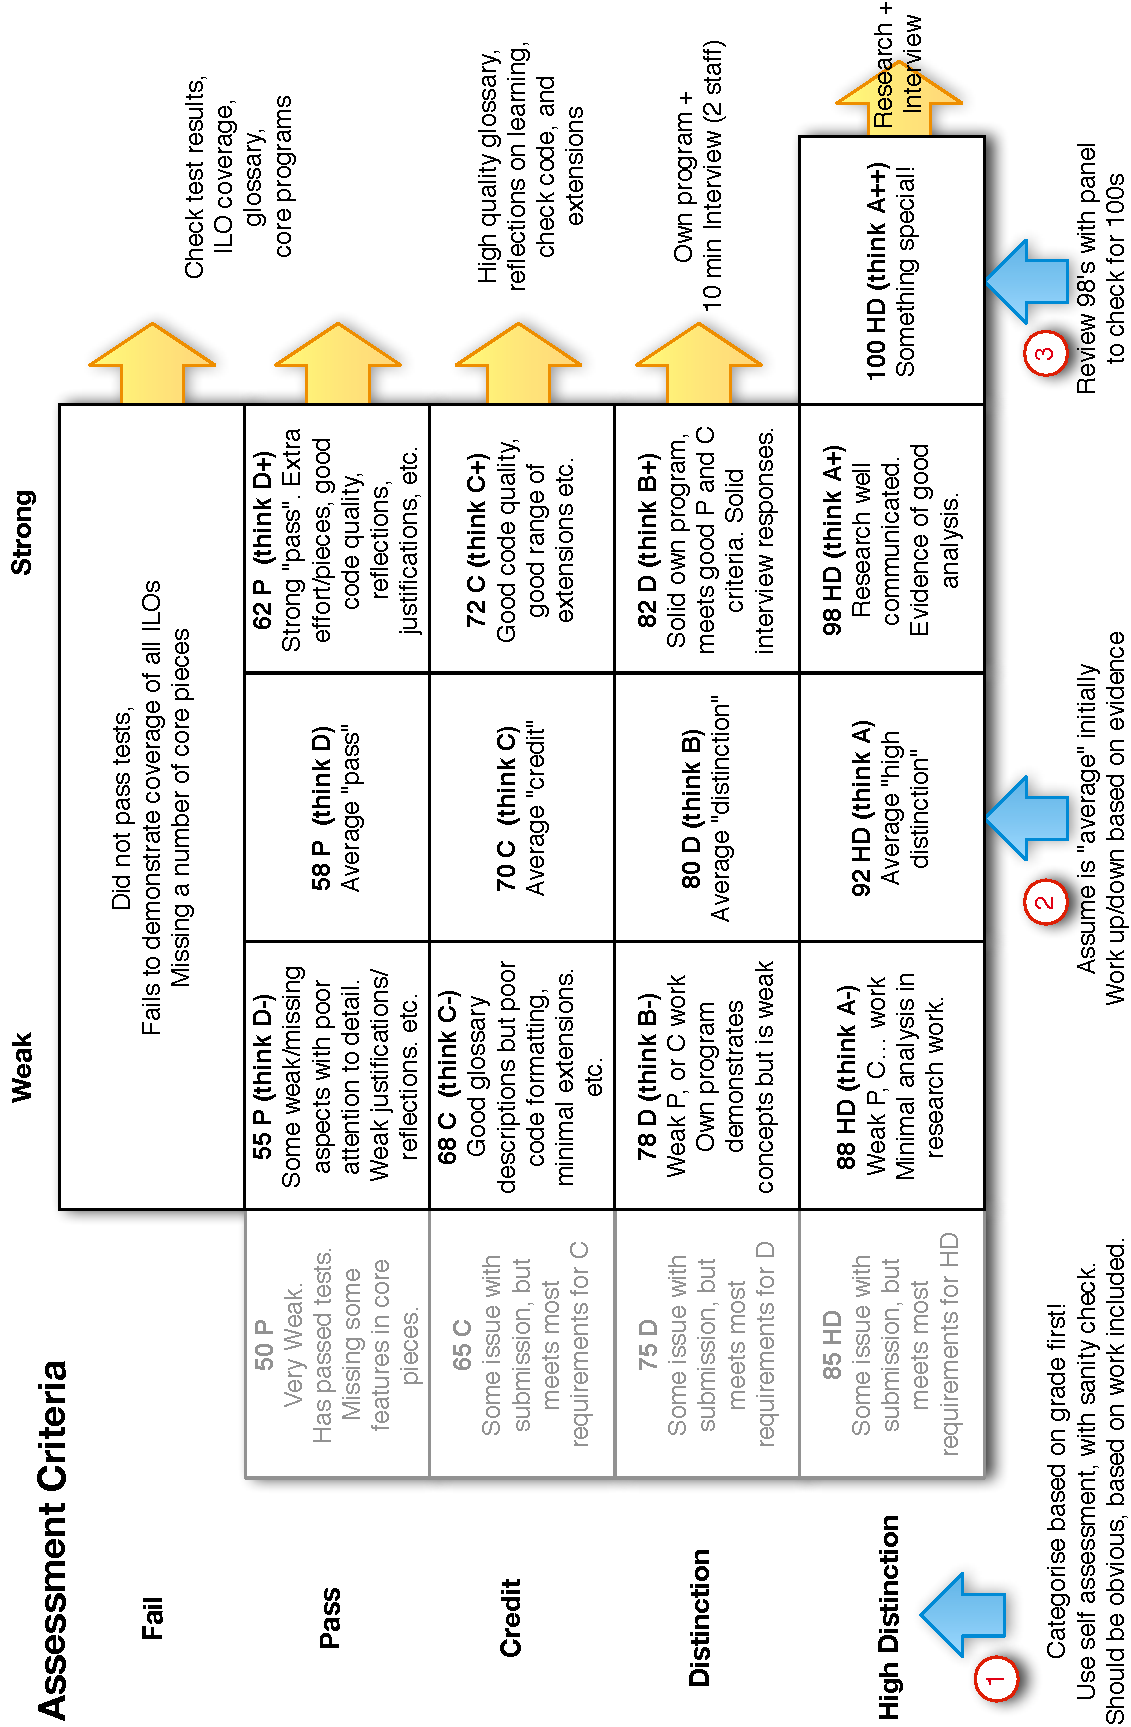
\includegraphics[width=0.98\textwidth]{AssessmentProcess}
	\caption{An overview of the assessment process used to explain the criteria to students.}
	\label{fig:assessment_process}
\end{figure}

The clearly distinct criteria for each grade made determining portfolio grades a simple task, with consistent outcomes. Pass criteria required students to have satisfactorily completed the hurdle tests, Credit required a good quality glossary and all work to be signed off, Distinction the custom project, and High Distinction the research report. 

For each of the grades the quality of the distinguishing artefacts needed to be checked against the expected standard. In the final portfolio assessment this task was greatly simplified due to the requirement for students to engage in the formative feedback process for Credit and higher grades. This meant that student work had already been checked by teaching staff, typically a number of times, before their portfolios were submitted. Any issues should have been identified and corrected before the final submission.

Students aiming for the Distinction and High Distinction grades were all interviewed. Each interview lasted around ten minutes, and was conducted by multiple teaching staff. In the interviews students were asked about their custom project and research work. The portfolio was used to guide the discussion, with screenshots and print outs of code often referred to. Overall the experience was very positive for students and staff, and provided staff with an opportunity to engage with the students who had achieved the most in the unit.

Assessing the students of the introductory programming unit in this way ensured all of the principles stated in \cref{cha:guiding_principles} were embedded throughout the unit.

\begin{itemize}[noitemsep,nolistsep]
	\item Assessment of portfolios aimed to assess the structure of the observed learning outcomes, as demonstrated in student portfolios. (\Pref{itm:construct})
	\item Portfolios had to demonstrate how the students' work aligned with \emph{all} of the unit's intended learning outcomes. (\Pref{itm:align})
	\item Final grades were based entirely on student portfolios, enabling frequent formative feedback to support student efforts during the unit delivery. (\Pref{itm:formative}, \Pref{itm:support} and \Pref{itm:theory_y})
	\item Assessment could focus on structured procedural programming concepts, as well as how they are realised in student programs. (\Pref{itm:focus}, \Pref{itm:paradigm} and \Pref{itm:concepts})
	\item Assessment criteria provided a clear message of high expectations, indicating what was required for students to achieve good grades. (\Pref{itm:expectations})
	\item Portfolios provided valuable evidence on the effectiveness of the learning environment, activities, and resources for staff reflections.  (\Pref{itm:agile} and \Pref{itm:reflect})
	\item Portfolios provided opportunities for students to reflect on their learning. (\Pref{itm:reflect})
	\item Programs created by students needed to demonstrate appropriate use of the programming languages used.  (\Pref{itm:authentic})
\end{itemize}

% subsection assessing_student_portfolios (end)
\subsection{Introductory Programming in Summary} % (fold)
\label{sub:intro_summary}

This section has presented an application of the model presented in \cref{cha:approach}, with the resulting unit encapsulating all of the principles from \cref{cha:guiding_principles}. The introductory programming unit was centred around its intended learning outcomes, and the central role of the student in constructing their own knowledge. The assessment criteria rewarded students for demonstrating a depth of knowledge, pushing students to strive for relational level understanding. Teaching and learning activities were developed to support the constructive nature of the unit, and to provide students with suitable challenges. The final summative assessment used assessment criteria and a specific process to quickly and efficiently determine student grade outcomes from the portfolios they submitted. 

\cref{cha:evaluation} and \cref{cha:discussion} provide further discussion of the results from delivering this unit.

In the next section another application of the model is presented in discussing the object oriented programming unit.

% subsection summary (end)

% section introductory_programming (end)
\clearpage
\section{Object Oriented Programming} % (fold)
\label{sec:object_oriented_programming}



\subsection{Aims for Object Oriented Programming} % (fold)
\label{sub:aims_for_object_oriented_programming}

Object oriented programming was the second programming unit in the sequence of programming units described in \sref{sec:paradigm_choice}. Having completed the introductory programming unit, many students went on enrol in the object oriented programming unit, which introduced them to the object oriented programming paradigm. 

The design of the object oriented programming unit followed the model outlined in \sref{sec:model} in a similar way to the introductory programming unit presented in \sref{sec:introductory_programming}. To help illustrate the general applicability of the model, this section briefly describes the steps taken and discusses how these differ from the approach taken with the introductory programming unit. The following subsections outline the processes from the model described in \sref{sec:model}, including the definition of the intended learning outcomes, construction of the assessment criteria, development of the teaching and learning activities, delivery of the unit, and portfolio assessment.

% subsection aims_for_object_oriented_programming (end)

\subsection{Defining Intended Learning Outcomes} % (fold)
\label{sub:oop_defining_intended_learning_outcomes}

Defining the object oriented programming unit's intended learning outcomes followed the same process as outlined for the introductory programming unit in \sref{sec:intro:intended_learning_outcomes}. The process was influenced by similar factors, and used the guidelines stated in \sref{sub:defining_intended_learning_outcomes}. The main difference between the object oriented programming unit and the introductory programming unit was the underlying programming paradigm. 

\pref{itm:paradigm} indicates that the strategy for delivering the unit should be founded on the programming paradigm being taught. The introductory programming unit covered procedural programming concepts, with the plan that the object oriented programming unit shift students to the object oriented programming paradigm, a shift that can be challenging for student \cite{Manns:1993,Sheetz:1997,White:2005}. In recognition of these challenges, the unit's intended learning outcomes focused on enabling students to make this shift in thinking.

To facilitate the paradigm shift the unit focused on the core principles underlying the object oriented programming paradigm: abstraction, encapsulation, inheritance, and polymorphism. Students learnt to use these principles to design and implement object oriented programs. In addition to the core principles, students learnt to use an integrated development environment (IDE), and unit testing tools such as JUnit \cite{JUnit}. Object oriented thinking and design were also central to the unit, with designs being communicated using Unified Modelling Language (UML) \cite{OMG:2011} class diagrams and sequence diagrams. While design patterns and heuristics provided students with a means of evaluating the quality of their designs.

The intended learning outcomes for the object oriented programming unit were:
\begin{guidelines}{ILO}
	\item \textbf{Explain} the principles of the object oriented programming paradigm specifically including abstraction, encapsulation, inheritance and polymorphism, and \textbf{explain} how these principles are used to create object oriented programs.
	\item \textbf{Design}, \textbf{develop}, \textbf{test}, and \textbf{debug} object oriented programs, using an integrated development environment.
	\item \textbf{Select} and \textbf{use} appropriate collection classes, from the language's class library, to manage collections of multiple objects.
	\item \textbf{Construct} appropriate diagrams and textual descriptions to \textbf{communicate} the static structure and dynamic behaviour of an object oriented solution.
	\item \textbf{Apply} accepted good practices related to the \textbf{construction} of object oriented programs.
\end{guidelines}

The following list shows how the guidelines for defining intended learning outcomes, stated in \sref{sub:defining_intended_learning_outcomes}, were used in the development of the object oriented programming unit.

\begin{itemize}[noitemsep,nolistsep]
	\item Verbs from the relational levels of the SOLO taxonomy were used to set appropriate levels of understanding. (\loref{lo-solo}) 
	\item Outcomes aimed to cover both an understanding of object oriented programming concepts and applied programming skills. (\loref{lo-know-prog})
	\item Simple terms were used to help ensure students were able to understand each outcome. (\loref{lo-simple-terms})
	\item Five outcomes were included, keeping the focus on a few key aspects. (\loref{lo-minimal})
	\item Outcomes were expressed in a general sense, enabling them to be met in a variety of ways and assessed at a range of levels of achievement. (\loref{lo-general} and \loref{lo-flex})
\end{itemize}

These guidelines helped with the formation of the intended learning outcomes for the object oriented programming unit, as they had introductory programming unit. The same general approach was taken, with differences in outcomes relating to the various unit focuses.

% subsection defining_intended_learning_outcomes (end)

\subsection{Constructing Assessment Criteria} % (fold)
\label{sub:oop_constructing_assessment_criteria}

The general nature of the assessment criteria from the introductory programming unit enabled these same criteria to be used for the object oriented programming unit. These did not need adjustment as each grade was described in a topic neutral manner. For example, for a Distinction students needed to ``demonstrate the \emph{application} of the unit's concepts to the creation of a program of their own design.'' This statement worked equally well for the object oriented programming unit as it did for the introductory programming unit. 

In essence, the assessment criteria described in \sref{sub:intro_constructing_assessment_criteria} aimed to ensure students had reached a relational level of understanding in order to achieve a Distinction or higher grade, and as a result the assessment criteria are likely to work for other technical software engineering units. Removing all topic specific details from these criteria results in criteria that could form the basis for a wide range of university units, as outlined in the following list.

\begin{description}[noitemsep,nolistsep]
	\item[Pass] is awarded to students who have done no more than meet the unit's minimum standards, as checked in weekly work or hurdle tests. 
	\item[Credit] is awarded to students who have demonstrated an integrated understanding of unit concepts, but have not demonstrated they can \emph{apply} the concepts to the creation of a piece of work of their own creation.
	\item[Distinction] is awarded to students who have demonstrated an integrated understanding of unit concepts, \textbf{and} have demonstrated they can \emph{apply} the concepts to the creation of a piece of work of their own creation.
	\item[High Distinction]  is awarded to students who have met the Distinction criteria and go beyond the scope of the unit in some way, such as through conducting a small research project.
\end{description}

The following list outlines how these general assessment criteria relate to the principles stated in \cref{cha:guiding_principles}.

\begin{itemize}[noitemsep,nolistsep]
	\item Students are encouraged to meet all intended learning outcomes, and to develop a relational level of understanding to achieve higher grades. (\Pref{itm:construct} and \Pref{itm:align})
	\item If portfolios determine all of a student's final grade then all summative assessment is delayed until the end of the unit. (\Pref{itm:formative})
	\item Student attention is focused on achievable steps at each level of the assessment criteria. (\Pref{itm:focus})
	\item Criteria for Distinction and High Distinction grades help communicate high staff expectations. (\Pref{itm:expectations})
	\item Simple terms help support a wide range of student language capabilities, helping to ensure students will understand what is required of them. (\Pref{itm:support})
	\item Use of clearly distinct requirements allow students to aim to meet certain grade criteria based on their personal interests and motivation. (\Pref{itm:theory_y})
	\item Frequent formative feedback encourages students to reflect on their learning and integrate feedback they receive. (\Pref{itm:agile} and \Pref{itm:reflect})
	\item Students needed to demonstrate appropriate application of concepts associated with the unit. (\Pref{itm:paradigm}, \Pref{itm:concepts} and \Pref{itm:authentic} in the case of introductory programming units)
\end{itemize}

% subsection constructing_assessment_criteria (end)

\subsection{Developing Teaching and Learning Activities, and Delivering the Unit} % (fold)
\label{sub:oop_developing_teaching_and_learning_activities}

Teaching and learning activities in the object oriented programming unit did differ from those in the introductory programming unit due to the altered focus of the unit. \sref{sec:paradigm_choice} outlined the programming concepts shared between procedural and object oriented programming, as illustrated in \tref{tbl:oo_proc_concepts}. This shows that object oriented programs and procedural programs share many features, and therefore many low level details do not need to be elaborated upon as students should be familiar with these concepts from the introductory programming unit. 

Object oriented programming involves constructing programs that consist of a number of interrelated object, with each object interacting with other objects to help achieve system goals. The thinking involved in designing object oriented programs, therefore, differs significantly from structured procedural programming. While the focus on the introductory programming unit had been on the internal implementation details of functions and procedure, the object oriented programming unit focused on modelling objects and designing object interactions. This required a different approach to unit teaching and learning activities.

As with the introductory programming unit, the guidelines stated in \sref{ssub:develop_teaching_and_learning_activities_and_resources} helped to shape the teaching and learning activities used. The activities aimed to actively engage students (\tlaref{itm:tla_active}), align with unit outcomes (\tlaref{itm:tla_align}), and provide guidance (\tlaref{itm:tla_focus}). These guidelines resulted in the use of the Beyond Bullet Points approach to presentations and object role-plays in lecture sessions, and the development of a number of case studies in laboratory classes.

Lectures were developed using the Beyond Bullet Points approach to ensure the focus was on concepts (\tlaref{itm:tla_focus} supporting \Pref{itm:focus} and \Pref{itm:concepts}). The short lecture presentations provided opportunities to engage students in more interactive activities in scheduled lecture times (\tlaref{itm:tla_active} supporting \Pref{itm:construct}). Where the introductory programming had made use of interactive code demonstrations, the object oriented programming used role-plays to focus students on object interactions, rather than language syntax (\Pref{itm:concepts}). In these role-plays students take on the role of objects in a program and send each other messages, simulating the objects students would later create in their code. Similar use of object role-plays was reported by \citet{Borstler:2005}, who found that they were beneficial in helping students understand object oriented concepts and thinking. 

The nature of object oriented paradigm means that it is best suited to developing larger solutions than those used in the introductory programming unit. The use of the object oriented programming principles, specifically inheritance and polymorphism, require a certain amount of infrastructure to see how these dramatically influence the way programs are designed. To help students engage with these principles, and to encourage students to develop greater learning independence, laboratory classes were adjusted to focus on a smaller number of programming problems that were larger than problems addressed in the introductory programming unit. These decisions were guided primarily by the chosen paradigm (\Pref{itm:paradigm}) and the need to ensure programs students create are an appropriate use of the chosen languages (\Pref{itm:authentic}).
 
A total of four programming ``case studies'' were used in the object oriented programming unit, two in the first half of the unit and a further two in the second half of the unit. One case study in each half of the teaching period was designed with significant guidance for students, and replaced the laboratory tasks that had been used in the introductory programming unit. The second case study required the application of the same principles, but with less guidance helping students to apply the concepts being learnt (\Pref{itm:construct}). UML diagrams were provided to explain the design of each case study, with iterations building relevant parts of the overall program. As the iterations progressed the details of the design were reduced, with students being required to design and implement the later iterations. 

Case studies supported students active role in the development of their knowledge and ensured students made appropriate use of the associated concepts (\tlaref{itm:tla_active} and \tlaref{itm:tla_focus} supporting \Pref{itm:construct}, \Pref{itm:paradigm}, \Pref{itm:concepts}, and \Pref{itm:authentic}). As with the introductory programming unit, the alignment was performed by both staff and students. Staff planned for the case studies to align with the unit's intended learning outcomes, and students related their individual learning to the outcomes in the preparation of their portfolios (\tlaref{itm:tla_align} supporting \Pref{itm:construct}, \Pref{itm:align} and \Pref{itm:concepts}).

\clearpage

In terms of alignment (\Pref{itm:align}) teaching staff planned for each case study to align with all of the intended learning outcomes, as shown in \tref{tbl:oop_matrix}. The following list indicates how the staff planned for each of the intended learning outcomes to relate to the case studies. Students were also required to indicate how they felt the pieces they had included in their portfolios aligned to the unit's intended learning outcomes, as was done in the introductory programming unit. 
\begin{itemize}[noitemsep,nolistsep]
	\item Students understanding of object oriented principles (ILO-1) was central to each case study, with students encouraged to reflect on how these principles were realised in the designs they implemented. 
	\item Each case study involved aspects of design, development, testing, and debugging (ILO-2) with students building functional programs. 
	\item The programs developed required students to use a range of classes from the languages' class libraries, including a variety of collection classes.
	\item Students needed to read as well as develop UML class and sequence diagrams in various parts of the case studies.
	\item Designs for the case studies demonstrated accepted good practice, and the iterative formative feedback process ensured students followed these, and associated, practices in their design and implementation tasks. Later case studies also introduced students to design patterns including the Composite and Command patterns \cite{Gamma:2001}.
\end{itemize}

\begin{table}[b]
	\centering
	\caption{Alignment matrix showing staff-planned alignment of case studies to the object oriented programming unit's intended learning outcomes. As with the introductory programming unit, student descriptions of the case study alignment differed based on their individual learning.}
	\label{tbl:oop_matrix}
	% \small
	\begin{tabular}{l|ccccc}
		\textbf{Topic} 								& \textbf{ILO-1} & \textbf{ILO-2} & \textbf{ILO-3} & \textbf{ILO4} & \textbf{ILO5} \\ \hline
		\emph{First Half} & & & & & \\
		~Case Study 1 - Drawing Program & \checkmark & \checkmark & \checkmark & \checkmark & \checkmark \\
		~Case Study 2 - Monopoly & \checkmark & \checkmark & \checkmark & \checkmark & \checkmark \\
		\hline
		\emph{Second Half} & & & & & \\
		~Case Study 3 - RPN Calculator & \checkmark & \checkmark & \checkmark & \checkmark & \checkmark \\
		~Case Study 4 - Text-based Adventure & \checkmark & \checkmark & \checkmark & \checkmark & \checkmark \\
	\end{tabular}
\end{table}

Core, and laboratory, tasks in the weekly work had students develop central object roles in the various case studies. These tasks were extended with optional extension tasks which were required in order to fully complete the programs described in the case studies. This helped communicate high expectations (\Pref{itm:expectations}) with all students being exposed to the full set of requirements and being encouraged to complete more than just the core tasks. As an example, \fref{fig:monopoly} shows a UML class diagram from the core tasks for the fourth iteration of the Monopoly case study, which focused on inheritance and polymorphism. Extension tasks associated with this iteration had students implement a ``Jail Tile'' and a ``Go To Jail Action''.

% In addition to learning the required aspects of the programming language, the case study introduced students to the Model View Controller (MVC) pattern. In core tasks students developed a command line interface to the program, with extension tasks adding a second graphical interface and thereby demonstrating the benefit of the MVC approach.

\begin{figure}[p]
	\centering
	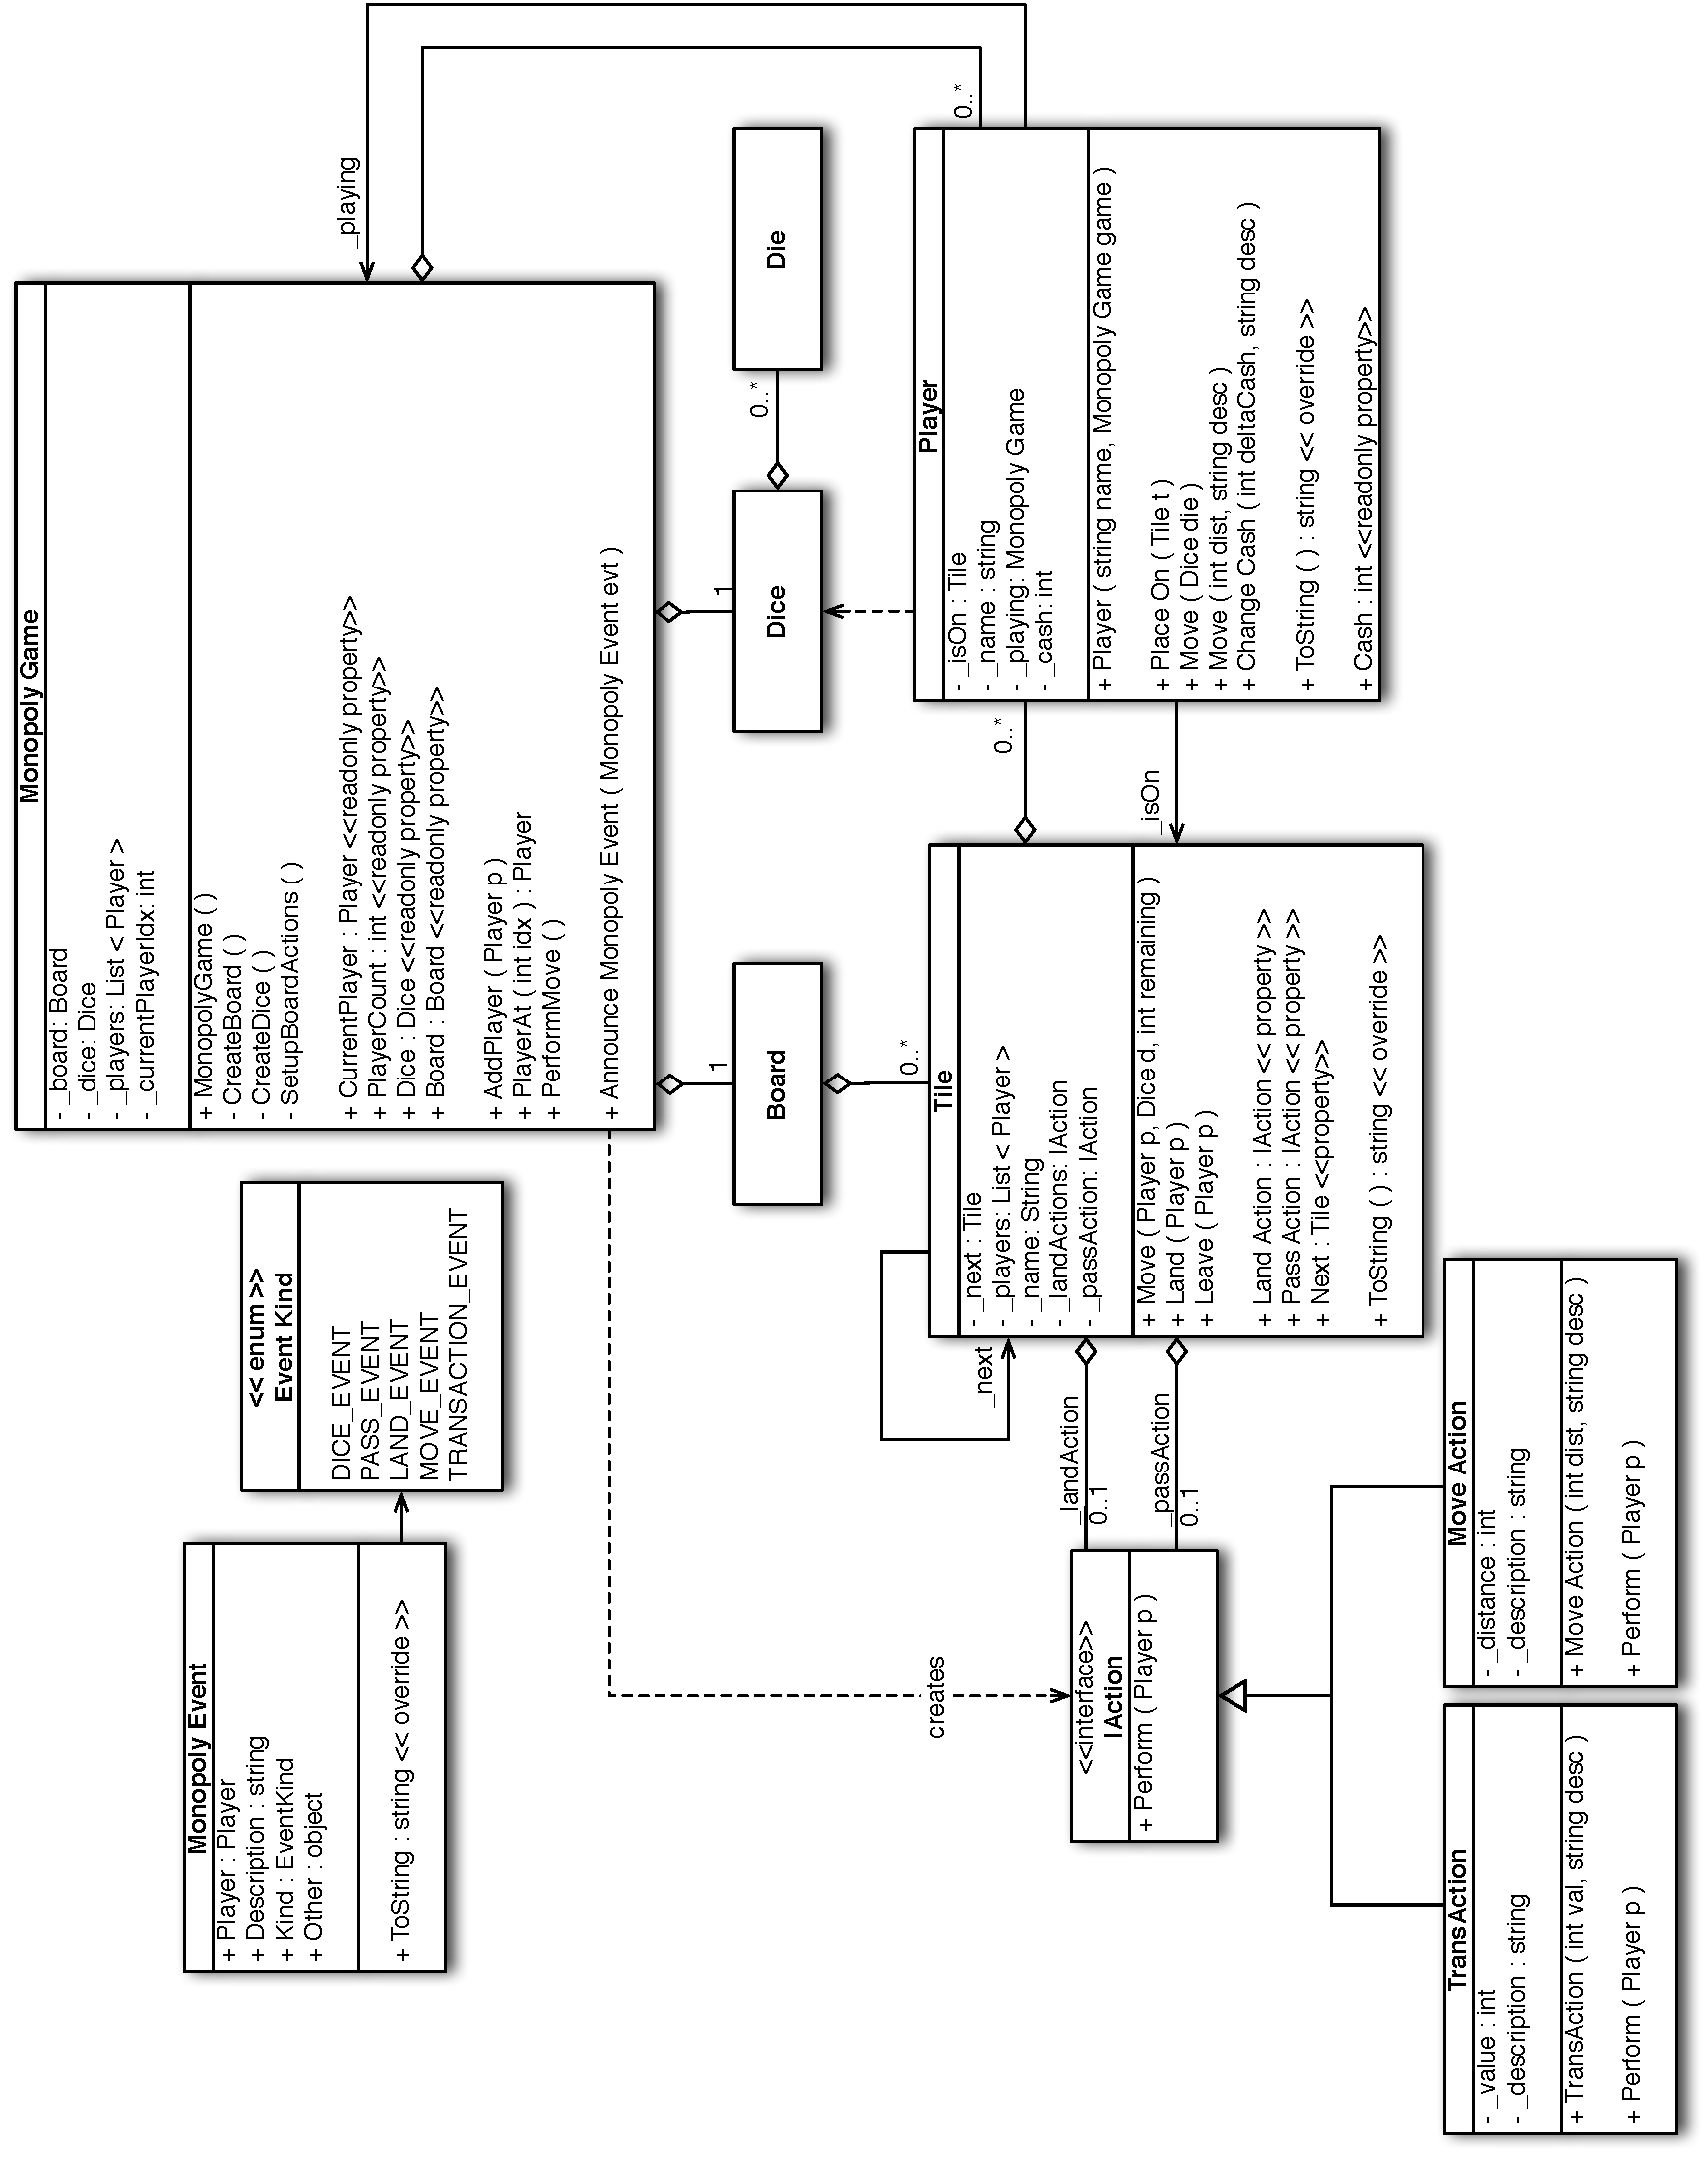
\includegraphics[width=\textwidth]{Monopoly1}
	\caption{An example UML class diagram from the Monopoly case study in the object oriented programming unit. }
	\label{fig:monopoly}
\end{figure}

Using such large case studies as the basis for the weekly tasks also helped to encourage students to think in terms of objects. Each case study started with an overall description of the final program, but built up the number of abstractions used each iteration to encourage this focus on object roles, responsibilities, and collaborations \cite{Wirfs:2003}.

% \begin{figure}[p]
% 	\centering
% 	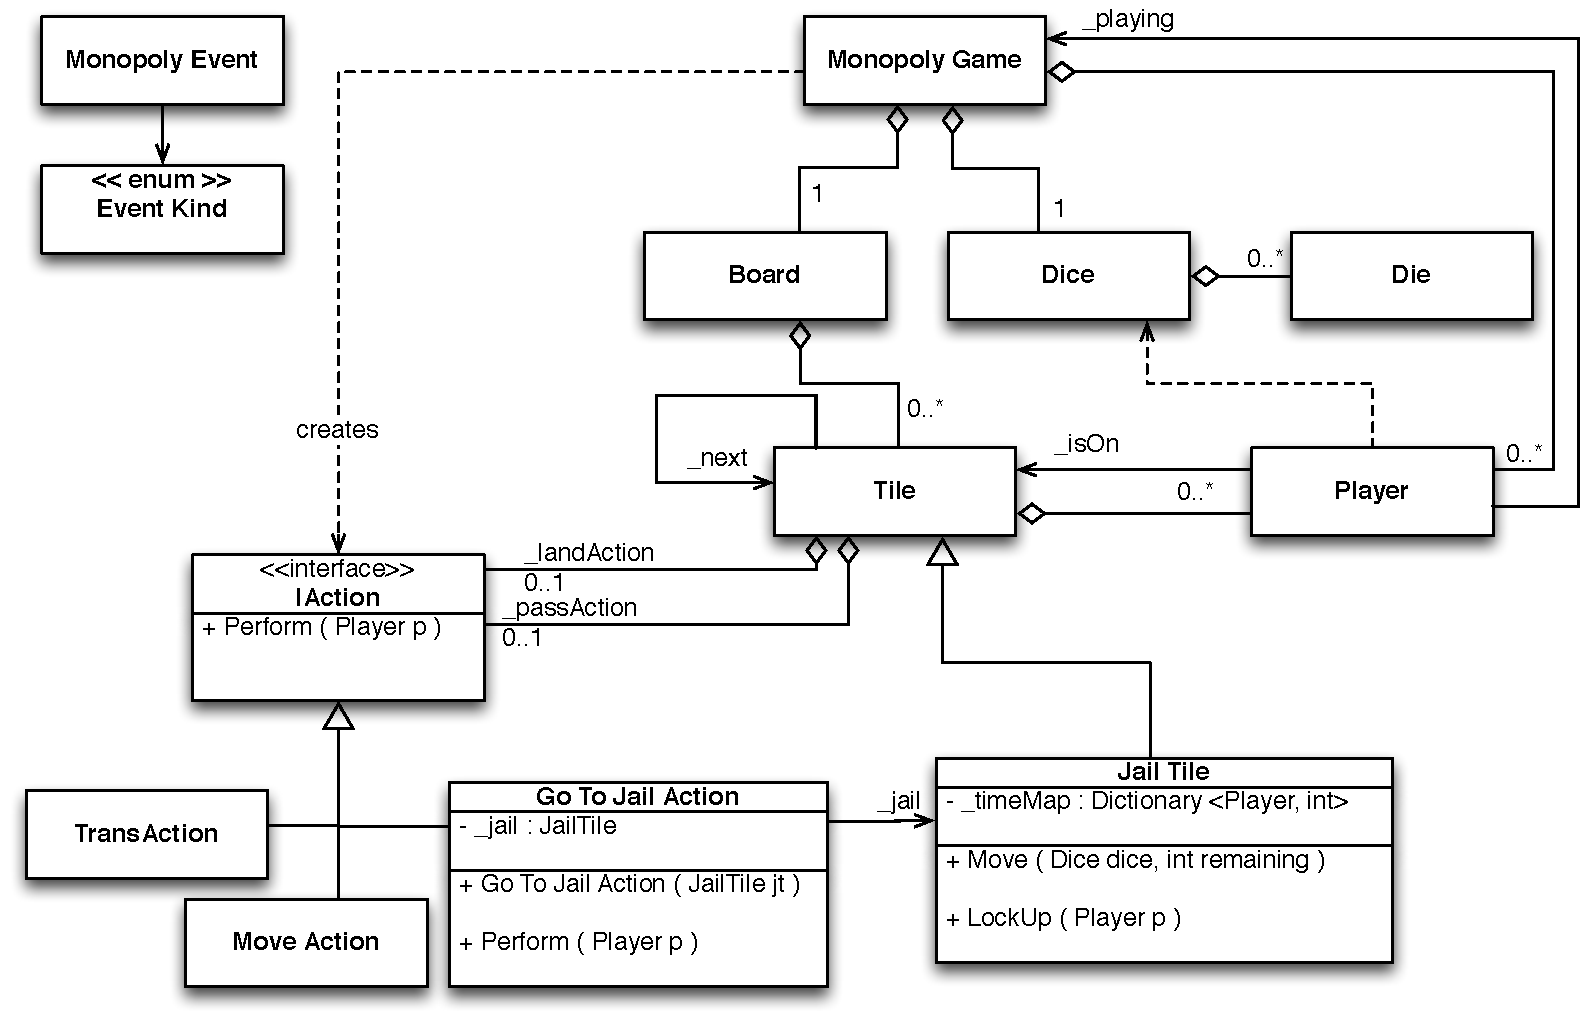
\includegraphics[width=\textwidth]{Monopoly}
% 	\caption{An example UML class diagram from the case studies in the object oriented programming unit demonstrating the relative complexity of the programs used to help students understand object oriented design issues}
% 	\label{fig:monopoly}
% \end{figure}

% As with the design aspects, the specification of the unit tests reduced over time with students taking full responsibility for designing the unit tests by the end of the case study.

Unit delivery followed the same iterative process as described for the introductory programming unit. Lectures were used to guide student activity, case studies had students apply concepts, weekly formative feedback assisted with student progress, and students incorporated feedback to improve their work and understanding. The following list outlines the similarities between the teaching and learning activities in the two programming units.

\begin{itemize}[noitemsep,nolistsep]
	\item Lectures focused on concepts, with role-plays taking the place of interactive coding demonstrations.
	\item Case studies formed the basis of the weekly laboratory, core, and optional tasks.

	\item Weekly tasks were submitted for formative feedback, and students were encouraged to incorporate the feedback they received.
	\item Staff discussed progress with each students weekly, and their work was signed off as complete after necessary feedback had been incorporated.
	\item The Programming Help Desk was available to support students outside of scheduled class times.
	\item Students were encouraged to use online discussion boards, with questions being monitored and answered by teaching staff and fellow students.
	\item A glossary was used alongside the case studies as a means for students to explain the concepts learnt.
\end{itemize}

The following list outlines how the object oriented programming unit's teaching and learning activities and delivery met all of the principles stated in \cref{cha:guiding_principles}.
\begin{itemize}[noitemsep,nolistsep]
	\item Case studies and lectures were designed to actively engage students in the construction of their own knowledge, providing guidance rather than aiming to transfer knowledge to students. (\Pref{itm:construct})
	\item Staff planned for lecture topics and case studies to align with the unit's intended learning outcomes, and students reflected on how these activities had aligned from their perspective. (\Pref{itm:align})
	\item Weekly tasks did not carry any weight in the final assessment, with learning outcomes being assessed from evidence included in student portfolios. (\Pref{itm:formative})
	\item Lectures focused on providing guidance, case studies on applying concepts, and support structures on providing assistance outside of scheduled class times. (\Pref{itm:focus})
	\item Case studies, with the associated core and extension tasks, helped communicate high staff expectations. (\Pref{itm:expectations})
	\item Students were actively supported during and outside of scheduled class times. (\Pref{itm:support})
	\item Students were trusted to manage their own learning, with no marks being associated with weekly work to ensure it remained focused on developing student understanding. (\Pref{itm:theory_y})
	\item Students and staff were encouraged to reflect on teaching and learning activities; students in terms of what they had learnt, and staff in terms of how well the activities had helped students understand the concepts. Staff reflections were used to alter subsequent delivery of the unit, while student were encouraged to incorporate reflections in the learning process. (\Pref{itm:agile} and \Pref{itm:reflect})
	\item Concepts related to the object oriented programming paradigm were central to all aspects of the unit. (\Pref{itm:paradigm} and \Pref{itm:concepts})
	\item Students developed object oriented programs using programming languages in ways in which they are intended to be used. (\Pref{itm:authentic})
\end{itemize}


\subsubsection{Choosing an Object Oriented Programming Language} % (fold)
\label{ssub:choosing_an_object_oriented_programming_language}

Another interesting aspect of the object oriented programming unit was the decision to allow students to choose which programming language they would use in the unit. By allowing students to choose their language, teaching staff were forced to discuss details at a conceptual level, making the unit clearly about object oriented programming and not the details of one specific language. 

While a wide variety of languages could be used in this unit, students were only provided with a choice between four programming languages: C\#, C++, Java and Objective-C. Each of these languages had a C-style syntax, helping ease students into the new syntax. C\#, Java and Objective-C had similar support for object oriented programming principles, with C++ being sufficient but requiring some extra attention to syntax to achieve the same outcomes. C\#, C++ and Java are statically typed, while Objective-C is dynamically typed. All had support from modern integrated development environments, and unit testing tools also required by the unit's intended learning outcomes.

Using multiple languages forced lectures, and laboratory class discussions, to focus on concepts (\Pref{itm:concepts}), while empowering students to choose a language they saw as relevant to their future careers (\Pref{itm:theory_y}). At the same time, the use of multiple languages enabled deeper exploration of concepts through the examination of how different languages implement object oriented features. For example, the difference between static and dynamic typing were discussed in lectures, and demonstrated to show different views on these concepts impact on program design. Similarly, different approaches to memory management were also discussed including manual memory management, reference counting, and garbage collection. In each case, these discussions focused on the general concepts and highlighted the various strengths and weaknesses of the various language implementations, providing a much richer learning experience than would have been possible with a single language.  

% The choice of language was guided by the following criteria:
% \begin{itemize}[noitemsep,nolistsep]
% 	\item Required a contemporary integrated development environment.
% 	\item Must support the object oriented programming paradigm.
% 	\item Must have unit testing tools.
% \end{itemize}

% Unlike introductory programming, in object oriented programming students selected one language and used this throughout the unit. 

Once again, the different languages helped strengthen the overall approach. This unit focused on object oriented programming, not on the specifics of a single language. The aim was not for students to develop a depth in \emph{one} programming language, but to learn the principles that underlie \emph{all} object oriented programming languages. Using multiple languages concurrently helped draw attention to this, and beneficially forced teaching staff to communicate at the concept level. 

% subsubsection choosing_an_object_oriented_programming_language (end)
% subsection developing_teaching_and_learning_activities (end)

\subsection{Assessing Student Portfolios} % (fold)
\label{sub:oop_assessing_student_portfolios}

As the assessment criteria were the same, the process of assessing student portfolios was the same as outlined for introductory programming. To pass, students had to satisfactorily complete two hurdle tests and demonstrate sufficient progress with the four case studies. Credit required a glossary that clearly documented the object oriented programming principles, and how they applied to programs the student had created. Distinction required a custom project that demonstrated the application of the object oriented programming principles, while High Distinction involved a research report. As with the introductory programming unit, students aiming for distinction and high distinction were interviewed as part of the assessment process.

Given the process was the same for assessing the object oriented programming unit, as it had been for the introductory programming unit, it too was able to embody all of the principles stated in \cref{cha:guiding_principles}.
\begin{itemize}[noitemsep,nolistsep]
	\item Portfolios were assessed to determine how well students understood object oriented programming concepts. (\Pref{itm:construct})
	\item Students needed to demonstrate how their work aligned with \emph{all} of the unit's intended learning outcomes. (\Pref{itm:align})
	\item Delivery involved an iterative process centred around formative feedback that supported student learning. (\Pref{itm:formative}, \Pref{itm:support} and \Pref{itm:theory_y})
	\item Object oriented programming principles and concepts were central to the entire process, including both delivery and assessment. (\Pref{itm:focus}, \Pref{itm:paradigm} and \Pref{itm:concepts})
	\item Case studies and assessment criteria aimed to clearly communicate high expectations. (\Pref{itm:expectations})
	\item Staff and students were involved in reflective practice, reflecting on past learning experiences to improve outcomes.  (\Pref{itm:agile} and \Pref{itm:reflect})
	\item Students developed a range of object oriented programs, demonstrating appropriate use of the languages they were expressed in.  (\Pref{itm:authentic})
\end{itemize}

% subsection assessing_student_portfolios (end)

% \subsection{Object Oriented Programming in Summary} % (fold)
% \label{sub:object_oriented_programming_in_summary}

% The object oriented programming unit presented here demonstrates a second application of the model presented in \cref{cha:approach}. As with the introductory programming unit, with the resulting unit encapsulated all of the principles from \cref{cha:guiding_principles}. The differences between the two units presented indicate the general applicability of the model.

% subsection object_oriented_programming_in_summary (end)

\subsection{Comparison with the Introductory Programming Unit} % (fold)
\label{sub:comparison_with_the_introductory_programming_unit}



% subsection comparison_with_the_introductory_programming_unit (end)

% subsection object_oriented_programming (end)

\clearpage
\section{Summary} % (fold)
\label{sec:ca_intro_summary}

This chapter provided two example implementations, in \sref{sub:introductory_programming} and \sref{sub:object_oriented_programming}, of the model described in \cref{cha:approach}. In each case the unit was developed and delivered using the processes discussed in \cref{cha:approach}, and was guided by the principles from \cref{cha:guiding_principles}. The described units have been delivery successfully across a number of teaching periods, and \cref{cha:evaluation} reports on the evaluation of these units while \cref{cha:discussion} discusses the relative importance of the various aspects of the approach overall.

In the following \cref{cha:supporting} we describe the teaching and learning resources that supported the delivery of these units.

% section summary (end)

% chapter constructively_aligned_introductory_programming_curriculum (end)